\documentclass[11pt]{article}
\usepackage[margin=1in]{geometry}
\usepackage{amsmath}
\usepackage{amssymb}
\usepackage{booktabs}
\usepackage{longtable}
\usepackage{hyperref}
\usepackage{microtype}
\usepackage{graphicx}
\usepackage{tikz}
\usepackage{quantikz}

\newcommand{\calV}{\mathcal{V}}
\newcommand{\Dt}{\Delta t}
\newcommand{\calH}{\mathcal{H}}
\newcommand{\calR}{\mathcal{R}}
\newcommand{\calL}{\mathcal{L}}
\newcommand{\calC}{\mathcal{C}}
\newcommand{\calP}{\mathcal{P}}
\newcommand{\Ht}{\tilde{H}}
\newcommand{\rhot}{\rho_t}
\renewcommand{\ket}[1]{\left| #1 \right\rangle}
\renewcommand{\bra}[1]{\left\langle #1 \right|}
\newcommand{\norm}[1]{\left\lVert #1 \right\rVert}
\newcommand{\Prep}{\mathrm{PREP}}
\newcommand{\Sel}{\mathrm{SEL}}
\DeclareMathOperator{\Tr}{Tr}

\title{Quantum resource estimation for fault-tolerant ZULF observable estimation}
\author{}
\date{}

\begin{document}
\maketitle

\section{Scope}

Notes toward a pipeline for quantum resource estimation (QRE) of
fault-tolerant algorithms that estimate local observables relevant to
ZULF (Zero/Ultra-Low Field) NMR spectroscopy.

\section{Background}
Our goal is to simulate the Lindblad equation
\begin{equation}
    \frac{d\rho}{dt} = \calL \rho = \calH \rho + \calR\rho
\end{equation}
where
\begin{align}
    \calH \rho &= -i\left[H,\rho\right]\\
    \calR \rho &= \sum_{j=1}^J L_j \rho L_j^\dagger -\frac{1}{2}\left\{L_j^\dagger L_j,\rho\right\}\label{eq:relaxation} 
\end{align}
The Lindblad equation implements the completely positive and trace-preserving (CPTP) map $\calV\left(t\right)=e^{\calL t}$. 
We will approximate the channel $\calV\left(t\right)$ by a channel
$\tilde{\calV}\left(t\right)=\tilde{\calV}^M_{\Dt}$ which splits the 
total time evolution into $M$ small steps of size $\Dt=t/M$.
$\tilde{\calV}_{\Dt}\left(\rho\right)$ channel can be implemented by appending $a_k$ ancilla 
qubits to the system in the state $\ket{0^{a_k}}$, time-evolving the
total system under an appropriate Hamiltonian $\tilde{H}$, and tracing out the ancilla.
The time-step evolution map is then given by
\begin{equation}
    \tilde{\calV}_{\Dt}\left(\rho\right) = \Tr_{a_k}\left\{\tilde{U}\left(\Dt\right)\rhot \tilde{U}^\dagger\left(\Dt\right)\right\},
\end{equation}
where $\tilde{U}\left(\Dt\right)=e^{-i\Dt \Ht}$, $\rhot=\ket{0^{a_k}}\bra{0^{a_k}}\otimes\rho$, and the dilated Hamiltonian is given as
\begin{equation}
    \Ht = \mathbf{1} \otimes H_0 + \Dt^{-1/2}\sum_{j=1}^{S_k}\left(\ket{j}\bra{0}\otimes L_j + \ket{0}\bra{j}\otimes L_j^\dagger\right)
\end{equation}


We can bound the error in the approximation as 
, where the trace distance (or Schatten 1-norm) is defined as 
$\norm{A}_1=\Tr\{\sqrt{A^\dagger A}\}$ for an operator $A$:
\begin{align}
    \norm{\calV\left(t\right)\rho - \tilde{\calV}\left(t\right)\rho}_1 &= \norm{\calV^M_{\Dt} \rho - \tilde{\calV}^M_{\Dt} \rho}_1\\
    &= \norm{\calV_{\Dt}\left(\calV^{M-1}_{\Dt}-\tilde{\calV}^{M-1}_{\Dt}\right) \rho + \left(\calV_{\Dt}-\tilde{\calV}_{\Dt}\right)\tilde{\calV}^{M-1}_{\Dt} \rho}_1\\
    &\leq \norm{\calV_{\Dt}\left(\calV^{M-1}_{\Dt}-\tilde{\calV}^{M-1}_{\Dt}\right) \rho}_1 + \norm{\left(\calV_{\Dt}-\tilde{\calV}_{\Dt}\right)\tilde{\calV}^{M-1}_{\Dt} \rho}_1\\
    &\leq \norm{\left(\calV^{M-1}_{\Dt}-\tilde{\calV}^{M-1}_{\Dt}\right) \rho}_1 + \norm{\left(\calV_{\Dt}-\tilde{\calV}_{\Dt}\right)\tilde{\calV}^{M-1}_{\Dt} \rho}_1\\
    &\le \norm{\left(\calV^{M-1}_{\Dt}-\tilde{\calV}^{M-1}_{\Dt}\right) \rho}_1+C_{k}\Dt^{k+1}\\
    &\vdots\\
    &\leq M C_{k}\Dt^{k+1}
\end{align}



where we have used $\norm{\left(\calV_{\Dt}-\tilde{\calV}_{\Dt}\right)\rho}\le C_{k} \Dt^{k+1}$ for any density operator $\rho$ and some $k\ge 1$ with a constant $C_{k}$ \cite{Ding2024}; the triangle inequality in the second line, the contractive property in the third line, and then repeated the argument. Thus, the error for the full evolution can be bounded as
\begin{equation}\label{eq:fullEvo_error}
    \norm{\calV\left(t\right)\rho - \tilde{\calV}\left(t\right)\rho}_1 \leq C_k t \Dt^k. 
\end{equation}

For a fixed timestep $\Dt$, we identify two sources of error in the approximation to the target Linbladian evolution:
\begin{align}\label{eq:err_deltT}
    \norm{\left(\calV_{\Dt}-\tilde{\calV}_{\text{trot},\Dt}\right)\rho} &= \norm{\left(\calV_{\Dt}-\tilde{\calV}_{\Dt}\right)\rho+\left(\tilde{\calV}_{\Dt}-\tilde{\calV}_{\text{trot},\Dt}\right)\rho}\\
    &\le \norm{\left(\calV_{\Dt}-\tilde{\calV}_{\Dt}\right)\rho}+\norm{\left(\tilde{\calV}_{\Dt}-\tilde{\calV}_{\text{trot},\Dt}\right)\rho}\\
    &\le \norm{\mathcal{P}_{\Dt}[\rho]}+2\norm{e^{-i\tilde{H}\Dt}-U_{\text{Trot}}}\\
    &=\epsilon_{\text{prf}}+2\epsilon_{\text{trot}}\\
    &=\epsilon_{\text{Tot}}
\end{align}
where $\mathcal{P}_{\Dt}[\rho]=\left(\calV_{\Dt}-\tilde{\calV}_{\Dt}\right)\rho$ for $\tilde{\calV}_{\Dt} = \text{Tr}_{\mathcal{A}}\{e^{-i\tilde{H}\Dt}\rho e^{i\tilde{H}\Dt}\}$ and 
\begin{equation}
\tilde{\calV}_{\text{trot},\Dt} = \text{Tr}_{\mathcal{A}}\{U_{\text{Trot},\Dt}\rho U^{\dagger}_{\text{Trot},\Dt}\},
\end{equation}
 $U_{\text{Trot},\Dt}$ encoding a Trotterized approximation to $e^{-i\tilde{H}\Dt}$. In going from the second to the third line, we used the contractive property of CPTP maps (the partial trace satisfying this condition) under the trace norm, together with:
 \begin{align}
     \norm{U\rho U^{\dagger}-V\rho V^{\dagger}}&\le \norm{U\rho\left(U^\dagger-V^{\dagger}\right)}+\norm{\left(U-V\right)\rho V^{\dagger}}\\
     &\le 2 \norm{U-V},
 \end{align}
 for unitaries $U,V$.
 \subsection{Observable-aware error}
 We now add the target observable into the picture. Let us define the error in 
 observable estimation for a single time step $\Dt$ as
 \begin{align}
    \delta\langle\hat{O}(\Dt)\rangle &= \text{Tr}\{\hat{O}\left(\calV_{\Dt}-\tilde{\calV}_{\text{trot},\Dt}\right)\rho\}\\
    &=\text{Tr}\{ \hat{O}\left(\calV_{\Dt}-\tilde{\calV}_{\Dt}\right)\rho+\hat{O}\left(\tilde{\calV}_{\Dt}-\tilde{\calV}_{\text{trot},\Dt}\right)\rho\}
 \end{align}
 where $\hat{O}$ is the observable of interest.

\subsubsection{Locality- and observable-weighted Trotter error}
\label{sec:trot_leading}

We now expand $\delta\langle\hat{O}(\Dt)\rangle_{\text{trot}}=\Tr\{\hat{O}\left(\tilde{\calV}_{\Dt}-\tilde{\calV}_{\text{trot},\Dt}\right)\rho\}$ to leading order in $\Dt$, exploiting that the ZULF observable $\hat{O}=\sum_iw_iS_i^+$ (the coil operator) and the coherent Hamiltonian $H_0$ are both built from low-weight (1- and 2-body) pieces.

\paragraph{Why coil is non-Hermitian, and why that is not a readout problem.} $\text{coil}=\sum_iw_iS_i^+$ is the standard NMR quadrature-detection observable: since $\rho(t)$ stays Hermitian under any (unitary or Lindbladian) evolution, $\Tr\{S_x^{\text{coll}}\rho(t)\}=\Re[\Tr\{\text{coil}\,\rho(t)\}]$ and $\Tr\{S_y^{\text{coll}}\rho(t)\}=\Im[\Tr\{\text{coil}\,\rho(t)\}]$ exactly, with $S_x^{\text{coll}}=\sum_iw_iS_{i,x}$, $S_y^{\text{coll}}=\sum_iw_iS_{i,y}$ -- so $\text{coil}$ packages two Hermitian quadrature channels into one complex signal. Dropping to a single Hermitian observable ($S_x^{\text{coll}}$ alone) is tempting but wrong for this protocol: unlike high-field NMR, where the analogous "which channel" question is about a rotating-frame carrier offset and the discarded channel is a physically irrelevant mirror far from the signal, ZULF has no carrier, and the J-coupling transition frequencies here are small and not sign-definite -- the unequal spin weights in $\rho_0$ and $\text{coil}$ are specifically what excite singlet--triplet coherences at $\pm J$, and discarding $S_y^{\text{coll}}$ symmetrizes $+J$ and $-J$ together, destroying the sign of the $J$-coupling (a genuine ZULF observable). The resolution is not to pick one Hermitian piece but to keep both: in Pauli terms $\text{coil}=S_x^{\text{coll}}+iS_y^{\text{coll}}$ with $S_x^{\text{coll}}=\tfrac12\sum_iw_iX_i$, $S_y^{\text{coll}}=\tfrac12\sum_iw_iY_i$ both Hermitian weight-1 Pauli sums, each directly estimable (no ancilla, no controlled-unitary, no Hadamard test), then combined classically as $\langle\text{coil}\rangle=\langle S_x^{\text{coll}}\rangle+i\langle S_y^{\text{coll}}\rangle$. The non-Hermiticity of $\hat{O}$ throughout this document is therefore a bookkeeping convenience (one complex trace instead of two real ones), not an obstacle to the resource-estimation pipeline's observable-readout gadget.

\paragraph{Elementary splitting.} Write $H_0=\sum_ph_p$, a sum of pairwise Heisenberg-coupling terms $h_{(k,l)}\propto J_{kl}\,\mathbf{S}_k\cdot\mathbf{S}_l$ and single-spin Zeeman terms $h_k$, each individually exponentiable. Together with one ancilla-coupling term per jump operator, $V_j=\ket{j}\bra{0}\otimes L_j+\ket{0}\bra{j}\otimes L_j^\dagger$, the dilated Hamiltonian splits as
\begin{equation}
    \tilde{H} = \sum_p\left(\ket{0}\bra{0}\otimes h_p\right)+\sum_{j=1}^{S_k}V_j,
\end{equation}
and $U_{\text{Trot}}=\prod_a e^{-i\tilde{H}_a\Dt}$ (first-order Lie--Trotter, over both families of terms in some fixed ordering).

\paragraph{Leading-order Trotter error operator.} For any splitting $\tilde{H}=\sum_a\tilde{H}_a$, a standard BCH expansion of the first-order product formula gives
\begin{equation}\label{eq:trot_leading_op}
    e^{-i\tilde{H}\Dt}-U_{\text{Trot}} = \frac{\Dt^2}{2}\calC+O(\Dt^3),\qquad \calC\equiv\sum_{a<b}\left[\tilde{H}_a,\tilde{H}_b\right],
\end{equation}
with $\calC^\dagger=-\calC$ (a commutator of Hermitian operators is anti-Hermitian).

\paragraph{Propagating $\delta U$ through the channel.} Write $\delta U\equiv e^{-i\tilde{H}\Dt}-U_{\text{Trot}}=\frac{\Dt^2}{2}\calC+O(\Dt^3)$, so $e^{-i\tilde{H}\Dt}=U_{\text{Trot}}+\delta U$. Substituting into the channel difference and expanding the product,
\begin{align}
    e^{-i\tilde{H}\Dt}\rhot e^{i\tilde{H}\Dt}-U_{\text{Trot}}\rhot U_{\text{Trot}}^\dagger
    &= \left(U_{\text{Trot}}+\delta U\right)\rhot\left(U_{\text{Trot}}+\delta U\right)^\dagger - U_{\text{Trot}}\rhot U_{\text{Trot}}^\dagger\\
    &= U_{\text{Trot}}\rhot\,\delta U^\dagger + \delta U\,\rhot U_{\text{Trot}}^\dagger + \delta U\,\rhot\,\delta U^\dagger.
\end{align}
The last term is $O(\Dt^4)$ (quadratic in $\delta U=O(\Dt^2)$) and is dropped. In the remaining two terms, $U_{\text{Trot}}=\mathbf{1}+O(\Dt)$, and since they already carry an explicit factor of $\delta U=O(\Dt^2)$, replacing $U_{\text{Trot}}\to\mathbf{1}$ there only omits an $O(\Dt)\times O(\Dt^2)=O(\Dt^3)$ correction -- beyond the order kept. This leaves
\begin{equation}
    e^{-i\tilde{H}\Dt}\rhot e^{i\tilde{H}\Dt}-U_{\text{Trot}}\rhot U_{\text{Trot}}^\dagger = \rhot\,\delta U^\dagger+\delta U\,\rhot+O(\Dt^3) = \frac{\Dt^2}{2}\left(\rhot\calC^\dagger+\calC\rhot\right)+O(\Dt^3).
\end{equation}
Using $\calC^\dagger=-\calC$, $\rhot\calC^\dagger+\calC\rhot=\calC\rhot-\rhot\calC=[\calC,\rhot]$, so
\begin{equation}
    e^{-i\tilde{H}\Dt}\rhot e^{i\tilde{H}\Dt}-U_{\text{Trot}}\rhot U_{\text{Trot}}^\dagger = \frac{\Dt^2}{2}\left[\calC,\rhot\right]+O(\Dt^3).
\end{equation}

\paragraph{Only the coherent splitting survives at this order.} $\rhot=\ket{0^{a_k}}\bra{0^{a_k}}\otimes\rho$ has ancilla support only in the ``00'' block, so $\Tr\{X\rhot\}$ depends only on the ancilla-diagonal (``00'') block of $X$, $\bra{0}X\ket{0}_a$. Every $V_j$ changes the ancilla index ($0\to j$ or $j\to0$), so: $[\ket{0}\bra{0}\otimes h_p,V_j]$ is purely ancilla off-diagonal (a $0\leftrightarrow j$ block), and $[V_j,V_k]$ for $j\neq k$ lives entirely in the ($j,k$)-nonzero ancilla sector -- both vanish upon restriction to the ``00'' block. Only commutators between two coherent pieces survive:
\begin{equation}\label{eq:C00}
    \bra{0}\calC\ket{0}_a = \sum_{p<q}[h_p,h_q]\equiv\calC_{00}.
\end{equation}
That is, \emph{to this order, the Trotter error in the observable estimate is controlled entirely by how $H_0$ is split into elementary exponentials} -- the choice of Trotter ordering/grouping for the dissipative (ancilla-coupling) gates does not contribute to $\delta\langle\hat{O}(\Dt)\rangle_{\text{trot}}$ until a higher order in $\Dt$.

\paragraph{Observable-projected leading error.} Combining the above,
\begin{equation}\label{eq:trot_leading_obs}
    \delta\langle\hat{O}(\Dt)\rangle_{\text{trot}} = \frac{\Dt^2}{2}\Tr\left\{\left[\hat{O},\calC_{00}\right]\rho\right\}+O(\Dt^3) = \frac{\Dt^2}{2}\sum_{p<q}\Tr\Big\{\big[\hat{O},[h_p,h_q]\big]\,\rho\Big\}+O(\Dt^3).
\end{equation}

\paragraph{Locality/weight pruning.} Since $\hat{O}=\sum_iw_iS_i^+$ is a sum of single-spin operators, $[\hat{O},X]=\sum_iw_i[S_i^+,X]$ vanishes term-by-term unless $X$ has nontrivial support on site $i$. Combined with the fact that $[h_p,h_q]\neq0$ only if $h_p,h_q$ share a spin (else they act on disjoint tensor factors and commute trivially), the double sum in Eq.~\eqref{eq:trot_leading_obs} collapses onto pairs of $H_0$-terms that (i) are mutually coupled on the spin graph and (ii) whose combined support reaches a nonzero-weight spin:
\begin{equation}\label{eq:trot_final}
    \big|\delta\langle\hat{O}(\Dt)\rangle_{\text{trot}}\big| \le \frac{\Dt^2}{2}\sum_i|w_i|\!\!\!\sum_{\substack{p<q\\ i\,\in\,\mathrm{supp}(h_p)\cup\mathrm{supp}(h_q)}}\!\!\!\big\|[S_i^+,[h_p,h_q]]\big\|_\infty+O(\Dt^3).
\end{equation}

Two remarks. First, Eq.~\eqref{eq:trot_final} is tighter than simply carrying through the earlier generic bound $2\epsilon_{\text{trot}}$: that bound triangle-inequalities the two cross terms $U_{\text{Trot}}\rhot\delta U^\dagger$ and $\delta U\rhot U_{\text{Trot}}^\dagger$ separately, whereas Eq.~\eqref{eq:trot_leading_obs} keeps their exact combination as a commutator, and the observable/locality restriction further prunes the sum to spin pairs actually coupled to (or overlapping the support of) a nonzero-weight spin. Second, since only $O(1)$ Heisenberg/Zeeman terms in $H_0$ overlap each spin $i$ (bounded by the local $J$-coupling/dipolar connectivity graph, not the total spin count), Eq.~\eqref{eq:trot_final} scales with the local coupling graph around the weighted spins rather than with the total number of terms in $\tilde{H}$ -- a genuinely QRE-relevant simplification, since it lets the Trotter-step budget for the coherent evolution be allocated based on local spin-graph structure around the $^{19}$F/weighted nuclei rather than the full system size.

\paragraph{Next order: the \texorpdfstring{$O(\Dt^3)$}{O(Dt\^{}3)} term.} Sec.~\ref{sec:nested_trot_numerics} shows that $K_{\text{trot}}$ -- the coefficient of the $\Dt^2$ term just derived -- vanishes identically for edge-colored Zeeman + isotropic-exchange splittings, so the actual leading behavior of $\delta\langle\hat{O}(\Dt)\rangle_{\text{trot}}$ is set by the next order in the same BCH expansion. Extending Eq.~\eqref{eq:trot_leading_op} one order further (verified by exact symbolic expansion of the truncated exponentials on both sides, checked against direct multiplication for $M=2$ and $M=3$ fragments with generic noncommuting Hermitian operators),
\begin{equation}\label{eq:trot_third_order}
    e^{-i\tilde{H}\Dt} - U_{\text{Trot}} = \frac{\Dt^2}{2}\calC + \Dt^3\calC^{(3)} + O(\Dt^4),
\end{equation}
where $\calC^{(3)}$ splits into a pairwise piece (one fragment appearing twice) and a genuinely three-fragment piece (three distinct fragments, the first place such a term can appear at this order):
\begin{align}
    \calC^{(3)} &= \sum_{a<b}\calC^{(3)}_{ab} \ +\ i\!\!\sum_{a<b<c}\!\Big(\{\tilde{H}_a,\tilde{H}_b,\tilde{H}_c\}_{\text{sym}} - \tilde{H}_a\tilde{H}_b\tilde{H}_c\Big),\label{eq:C3_split}\\
    \calC^{(3)}_{ab} &\equiv -\frac{i}{4}\Big([\tilde{H}_a^2,\tilde{H}_b]+[\tilde{H}_a,\tilde{H}_b^2]\Big) - \frac{i}{12}\Big([\tilde{H}_a,[\tilde{H}_a,\tilde{H}_b]]+[\tilde{H}_b,[\tilde{H}_b,\tilde{H}_a]]\Big),\label{eq:C3_pair}
\end{align}
with $\{A,B,C\}_{\text{sym}}\equiv\frac16\big(ABC+ACB+BAC+BCA+CAB+CBA\big)$ the fully symmetrized triple product (sum over all $3!$ orderings). Both pieces are built entirely from products of two or three of the original fragments $\tilde{H}_a$ -- $\calC^{(3)}$ has exactly the same kind of support structure as $\calC$, just one fragment deeper, so the same style of locality/observable-weight pruning used to reach Eq.~\eqref{eq:trot_final} applies again here, now over pairs and triples of mutually- (or chain-) coupled fragments overlapping a nonzero-weight spin. The corrected scaling is
\begin{equation}
    \delta\langle\hat{O}(\Dt)\rangle_{\text{trot}} = O(\Dt^3)
\end{equation}
for the edge-colored Zeeman + isotropic-exchange systems considered here -- one power of $\Dt$ better than the generic first-order-Trotter estimate. This pure-coherent term is not, however, the whole next-order story: it treats every jump operator $V_j$ as an exact atomic exponential, whereas the real circuit \emph{also} Trotterizes each $V_j$ into its own Pauli terms (Sec.~\ref{sec:nested_trot_leading}). Combining the two layers produces genuine cross terms between coherent and nested fragments that neither analysis alone captures, worked out in Sec.~\ref{sec:combined_trot_nested}.

\subsubsection{Leading-order purification error}
\label{sec:prf_leading}

We now expand $\delta\langle\hat{O}(\Dt)\rangle_{\text{prf}}=\Tr\{\hat{O}\left(\calV_{\Dt}-\tilde{\calV}_{\Dt}\right)\rho\}$ to leading order in $\Dt$, using the corrected dilation $\tilde{U}(\Dt)=e^{-i\Dt\Ht}$, $\Ht=\mathbf{1}\otimes H_0+\Dt^{-1/2}\sum_jV_j$.

\paragraph{Kraus expansion.} Writing $\theta\equiv\sqrt{\Dt}$, $A\equiv\mathbf{1}\otimes H_0$, $B\equiv\sum_jV_j$, the dilated evolution operator is $\tilde{U}(\theta)=e^{-i\theta B-i\theta^2A}$, and $\tilde{\calV}_{\Dt}(\rho)=\sum_mK_m(\theta)\rho K_m^\dagger(\theta)$ with $K_m(\theta)=\bra{m}\tilde{U}(\theta)\ket{0}_a$. Expanding order by order in $\theta$ and using that $B$ has no ancilla self-loops (it only connects ancilla index $0\leftrightarrow j$) while $A$ is exactly ancilla-diagonal, one finds by direct computation that \emph{$K_0$ contains only even powers of $\theta$ and each $K_j$ only odd powers} -- a parity property of the ancilla-hopping graph, not a coincidence of any particular order. Concretely, through the order needed below (with $\Gamma\equiv\sum_jL_j^\dagger L_j$),
\begin{align}
    K_0(\theta) &= \mathbf{1}+\theta^2k_2+\theta^4k_4+O(\theta^6), & k_2&=-iH_0-\tfrac12\Gamma,\\
    K_j(\theta) &= \theta(-iL_j)+\theta^3\kappa_j+O(\theta^5), & \kappa_j&=-\tfrac12\{H_0,L_j\}+\tfrac i6L_j\Gamma,
\end{align}
\begin{equation}
    k_4 = -\tfrac12H_0^2+\tfrac i6\Big(H_0\Gamma+\textstyle\sum_kL_k^\dagger H_0L_k+\Gamma H_0\Big)+\tfrac1{24}\Gamma^2.
\end{equation}
Because $\theta=\sqrt{\Dt}$ and only even powers of $\theta$ survive in $\tilde{\calV}_{\Dt}(\rho)=K_0\rho K_0^\dagger+\sum_jK_j\rho K_j^\dagger$ (even$\times$even from $K_0$, odd$\times$odd from the $K_j$), \emph{$\tilde{\calV}_{\Dt}(\rho)$ is analytic in integer powers of $\Dt$ with no leftover half-integer terms} -- this is the structural fix relative to the earlier dilation, where $H_0$ entering at $O(\theta)$ produced a spurious $O(\sqrt{\Dt})$ term.

\paragraph{Leading-order coefficient.} Collecting the $\theta^4=\Dt^2$ terms,
\begin{equation}\label{eq:R_rho}
    \tilde{\calV}_{\Dt}(\rho) = \rho+\Dt\,\calL[\rho]+\Dt^2R[\rho]+O(\Dt^3),\qquad R[\rho] = k_4\rho+\rho k_4^\dagger+k_2\rho k_2^\dagger+\sum_j\Big(-iL_j\rho\kappa_j^\dagger+i\kappa_j\rho L_j^\dagger\Big),
\end{equation}
which matches $e^{\Dt\calL}[\rho]=\rho+\Dt\calL[\rho]+\frac{\Dt^2}{2}\calL^2[\rho]+O(\Dt^3)$ through $O(\Dt)$, so the leading purification error is
\begin{equation}\label{eq:Cprf}
    \calP_{\Dt}[\rho] = \Dt^2\,C_{\text{prf}}[\rho]+O(\Dt^3),\qquad C_{\text{prf}}[\rho]\equiv R[\rho]-\tfrac12\calL^2[\rho].
\end{equation}
As a check, when every $L_j=0$ (purely coherent system), $\Gamma\to0$, $\kappa_j\to0$, $k_2\to-iH_0$, $k_4\to-\tfrac12H_0^2$, and $R[\rho]\to-\tfrac12H_0^2\rho-\tfrac12\rho H_0^2+H_0\rho H_0=-\tfrac12[H_0,[H_0,\rho]]$, which exactly cancels $\tfrac12\calL^2[\rho]\to-\tfrac12[H_0,[H_0,\rho]]$ -- as it must, since $\tilde{H}$ reduces to $\mathbf{1}\otimes H_0$ with no dissipative coupling and $\tilde{\calV}_{\Dt}=\calV_{\Dt}$ exactly in that limit. Eq.~\eqref{eq:R_rho}--\eqref{eq:Cprf} were additionally verified numerically: on a random $2$-qubit test system ($H_0$, two jump operators $L_1,L_2$ Haar-random), the trace-norm error $\|\calP_{\Dt}[\rho]\|_1$ (against an independent high-accuracy RK4 integration of the exact Lindbladian) shows a local log-log slope converging to $2.00$ as $\Dt\to0$, and the Richardson-extrapolated coefficient $\calP_{\Dt}[\rho]/\Dt^2$ agrees with $C_{\text{prf}}[\rho]$ evaluated from Eq.~\eqref{eq:Cprf} to a relative error of $\sim10^{-4}$ (consistent with the extrapolation's own truncation).

\paragraph{Observable-projected leading error.}
\begin{equation}\label{eq:prf_leading_obs}
    \delta\langle\hat{O}(\Dt)\rangle_{\text{prf}} = \Dt^2\,\Tr\{\hat{O}\,C_{\text{prf}}[\rho]\}+O(\Dt^3).
\end{equation}

\paragraph{Why the trot-style locality pruning does not carry over.} In the trot analysis, the leading error was $[\calC,\rho]=\calC\rho-\rho\calC$ -- a commutator with the \emph{same} operator $\calC$ on both sides, so cyclicity gave $\Tr\{\hat{O}[\calC,\rho]\}=\Tr\{[\hat{O},\calC]\rho\}$, and $[\hat{O},\calC]$ vanishes \emph{as an operator identity} wherever $\calC$ has no support -- true for any $\rho$. Here, $R[\rho]$ is built from genuine sandwich terms $A\rho B$ with $A\neq B$ (e.g.\ $k_4\rho$, $L_j\rho\kappa_j^\dagger$), the generic GKSL structure. Cyclicity gives $\Tr\{\hat{O}A\rho B\}=\Tr\{(B\hat{O}A)\rho\}$, but $B\hat{O}A$ need not vanish just because $A,B$ miss some site $i$: if $\rho$ itself is entangled across that site, $\Tr\{(B\hat{O}A)\rho\}$ picks up $\rho$'s own correlations there and is generically nonzero. \emph{The exact support-pruning that made the trot bound tight is special to commutator structures and does not apply to the prf error's leading term.}

\paragraph{Resulting (weaker, but still local) bound.} What survives is locality at the level of operator norms: $H_0=\sum_ph_p$ and each $L_j$ are individually 1-/2-body, so $\Gamma=\sum_jL_j^\dagger L_j$ and the composite operators in $k_2,k_4,\kappa_j$ are sums of bounded-support pieces, and submultiplicativity of $\|\cdot\|_\infty$ together with $\|\rho\|_1=1$ gives
\begin{equation}\label{eq:prf_final}
    \big|\delta\langle\hat{O}(\Dt)\rangle_{\text{prf}}\big| \le \Dt^2\,\|\hat{O}\|_\infty\left(\|k_4\|_\infty+\tfrac12\|k_2\|_\infty^2+\sum_j\|L_j\|_\infty\|\kappa_j\|_\infty+\tfrac12\|\calL^2\|_{\infty\to\infty}\right)+O(\Dt^3),
\end{equation}
with $\|\hat{O}\|_\infty\le\sum_i|w_i|$ and each $\|k_4\|_\infty,\|\kappa_j\|_\infty$ bounded in turn by the triangle inequality on their constituent low-body terms ($\|H_0\|_\infty$, $\|L_j\|_\infty$, $\|\Gamma\|_\infty\le\sum_j\|L_j\|_\infty^2$), all directly computable from the existing Pauli-string pipeline. Unlike Eq.~\eqref{eq:trot_final}, this does \emph{not} restrict to a local neighborhood of the nonzero-weight spins -- it scales with the \emph{global} operator norms of $H_0$ and $\Gamma$, which for an extensive $N$-spin system with bounded per-term couplings grow at worst linearly in $N$ (via the triangle inequality over local terms), rather than being suppressed to $O(1)$ terms near the weighted nuclei. This is a genuine asymmetry between the two error sources: \emph{the trot budget can be allocated locally around the observable; the prf budget cannot, at least not without a sharper (non-operator-norm) argument than the one used here.}

\section{Numerical verification: prf vs.\ trot error scaling on truncated Gemcitabine}
\label{sec:numerical_verification}

To build intuition for how $\delta\langle\hat{O}(\Dt)\rangle_{\text{prf}}$ and $\delta\langle\hat{O}(\Dt)\rangle_{\text{trot}}$ actually scale with $\Dt$ -- and to check the leading-order analytics of Secs.~\ref{sec:trot_leading}--\ref{sec:prf_leading} against a fully numerically-exact reference -- both quantities were computed on a small, tractable test system: the truncated 5-spin Gemcitabine ZULF model (F0, F1, H2, H3, C0; $D=32$), using the precomputed coherent Hamiltonian and canonical jump operators in \texttt{circ\_sim/scripts/gemcitabine\_trunc/data/gemcitabine\_5spin\_krylov\_ops.pkl} (Krylov order 0, i.e.\ undressed canonical $L_j$, matching the rest of this document). Of the 34 canonical jump operators only the 25 rank-2 operators are numerically nonzero for this system (the 9 rank-1 operators vanish identically, as in the fluo\_suite systems discussed elsewhere), so $S_k=25$ and the ancilla dimension is $26$.

\paragraph{Trotterization scheme.} The coherent part $H_0=H_Z+H_J$ (Zeeman + pairwise Heisenberg coupling) is split as: a single fused Zeeman layer (all single-spin terms commute exactly, applied first), followed by Heisenberg-coupling layers obtained from a greedy edge coloring of the $J$-coupling graph -- the standard technique for Trotterizing Heisenberg-type Hamiltonians, since two-body exchange terms on disjoint qubit pairs commute exactly and fuse into a single native gate per color class, with commutativity between bonds determined purely by vertex-disjointness on the coupling graph (no general Pauli-commuting-set search needed, unlike the dense/high-weight case in chemistry VQE measurement grouping) -- ordered by decreasing summed $|J|$ (rad/s) within each class, strongest coupling first. The dissipative part is applied after the full coherent part, as 25 individual exponentials $\exp(-i\sqrt{\Dt}\,V_j)$, in one of two independently-generated random orderings (``A'' and ``B''), to check the analytically-predicted insensitivity of the trot error to jump-operator ordering.

\paragraph{Reference channels.} For each $\Dt$, three channels are propagated from the same ZULF initial state $\rho_0$ (sudden-transfer high-temperature state $\rho_{\text{sud}}=\sum_nw_nS_{n,z}$ followed by a $\pi/2$ pulse about $y$, $w_n=\gamma_n/\gamma_{^1\text{H}}$) for $M=1,\ldots,10$ steps ($t=M\Dt$):
\begin{itemize}
    \item the \emph{exact} Lindbladian channel $\calV(t)=e^{t\calL}$, via eigendecomposition of the full $D^2\times D^2$ Liouvillian;
    \item the \emph{exact-dilation} channel $\tilde{\calV}_{\Dt}^M$, iterating the exact (non-Trotterized) dilated-Hamiltonian map;
    \item the \emph{Trotterized-dilation} channel $\tilde{\calV}_{\text{trot},\Dt}^M$, iterating the first-order Lie--Trotter product described above, for both jump-operator orderings.
\end{itemize}
At each $t=M\Dt$, $\delta\langle\hat{O}(t)\rangle_{\text{prf}}=\Tr\{\hat{O}(\calV(t)-\tilde{\calV}_{\Dt}^M)\rho_0\}$ and $\delta\langle\hat{O}(t)\rangle_{\text{trot}}=\Tr\{\hat{O}(\tilde{\calV}_{\Dt}^M-\tilde{\calV}_{\text{trot},\Dt}^M)\rho_0\}$, with $\hat{O}=\text{coil}=\sum_iw_iS_i^+$ (non-Hermitian; only $|\delta\langle\hat{O}(t)\rangle|$ is shown). The relative error $|\delta\langle\hat{O}(t)\rangle|/|\langle\hat{O}(t)\rangle|$ is plotted, normalizing out the (oscillating, decaying) magnitude of the FID signal itself.

\paragraph{Step-size sweep.} $\delta_t\equiv1/(2|J_{F0\text{-}C0}|)\approx2.204$~ms (the larger of the two F--C $J$-couplings in this system's CF$_2$ group) sets two nested sweeps of five $\Dt$ values each, $\{1,3,5,7,9\}\times\delta_t$ and $\{1,3,5,7,9\}\times\delta_t/50$, ten values in total, each run for the same 10 Trotter steps.

\begin{figure}[h]
    \centering
    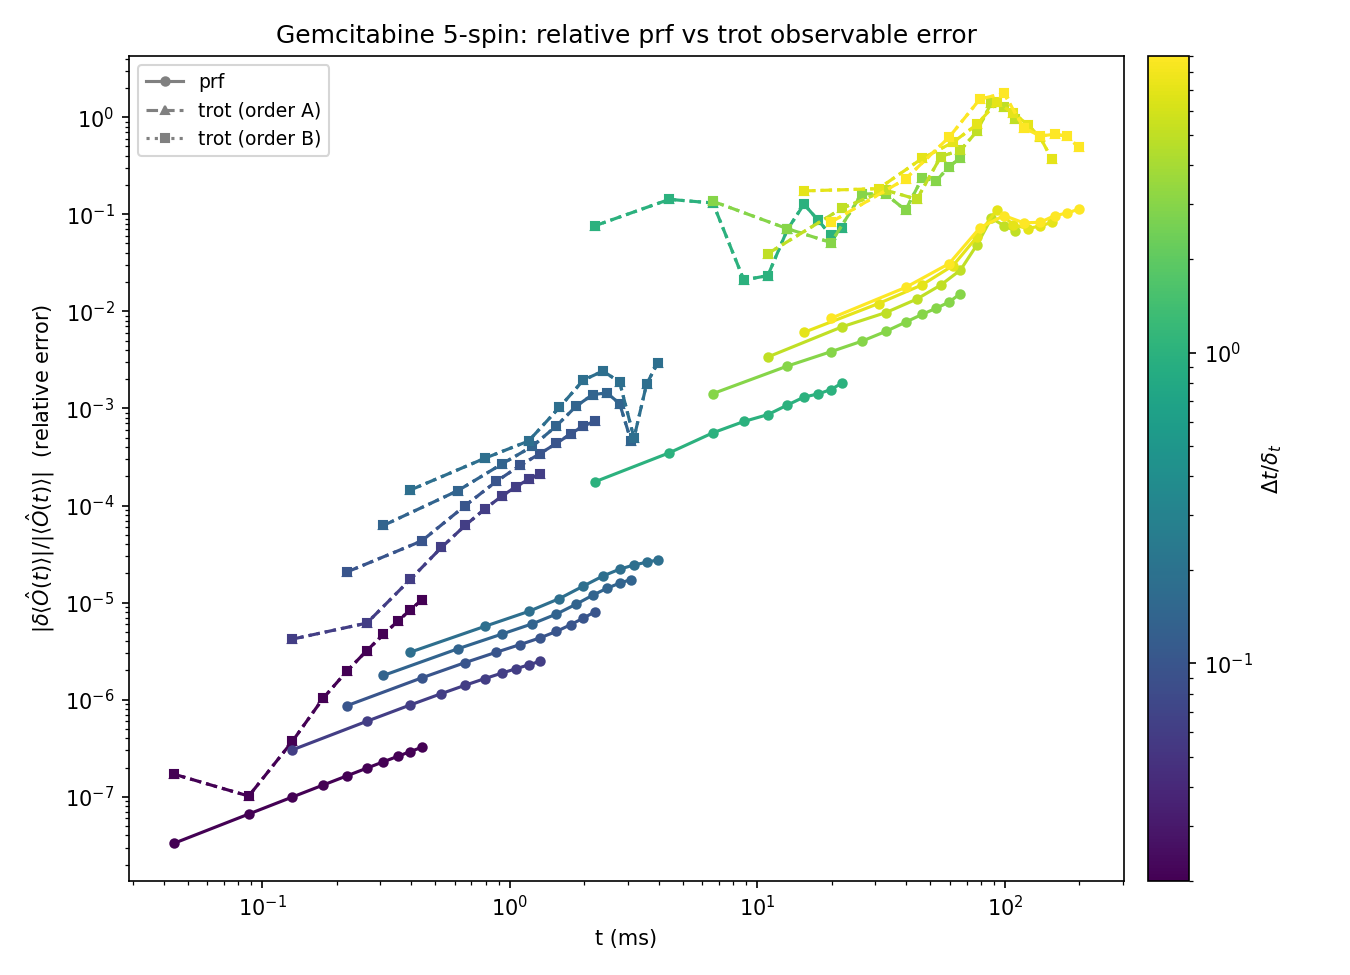
\includegraphics[width=0.85\textwidth]{../data/trotter_prf_vs_trot_gemcitabine5.png}
    \caption{\label{fig:prf_vs_trot}Relative observable error $|\delta\langle\hat{O}(t)\rangle|/|\langle\hat{O}(t)\rangle|$ vs.\ time, for the prf channel (solid, circles) and the trot channel at both jump-operator orderings (dashed/dotted, triangles/squares), colored by $\Dt/\delta_t$ on a log scale. Ten $\Dt$ values, $M=1$--$10$ steps each.}
\end{figure}

\paragraph{Findings.} (i) A single-step scan down to $\Dt=10^{-3}\delta_t$ confirms both error sources approach their analytically-derived leading order: the prf local log-log slope converges cleanly to $2.00$ already by $\Dt\sim10^{-2}\delta_t$, while the trot slope converges to the same $O(\Dt^2)$ scaling only much more slowly ($3.79\to2.26$ over the same range) -- consistent with $\delta_t$ being comparable to, not smaller than, the fastest coherent oscillation period in this system (itself set by $J_{F0\text{-}C0}$), so the coherent (trot) part needs a much smaller step before its leading-order term dominates. (ii) This is directly visible in Fig.~\ref{fig:prf_vs_trot}: the small-$\Dt$ curves ($\Dt/\delta_t\lesssim0.2$, dark) trace smooth, near-power-law relative-error curves for both prf and trot, while the original $\Dt\sim\delta_t$ curves (bright) show trot developing visible non-monotonic structure (bumps/dips from beating between the exact and Trotterized coherent phases) rather than clean decay. (iii) Across the \emph{entire} range tested, prf and trot separate into two consistent bands roughly two orders of magnitude apart, trot dominating -- the Trotter (coherent-splitting) error is the larger contributor to the total algorithmic error for this system at these step sizes, not the purification/dilation error. (iv) The two jump-operator orderings (A, B) agree to 3--4 significant figures throughout, confirming the trot error's predicted insensitivity to jump-operator ordering (Sec.~\ref{sec:trot_leading}).

Reproducible via \texttt{circ\_sim/scripts/QRE/trotter\_prf\_vs\_trot\_gemcitabine5.py}, which regenerates both the data (\texttt{data/trotter\_prf\_vs\_trot\_gemcitabine5.pkl}) and Fig.~\ref{fig:prf_vs_trot}.

\section{Algorithmic gadget: block-encoding a single jump-operator term \texorpdfstring{$e^{-i\sqrt{\Dt}\,V_j}$}{e\^{}(-i sqrt(Dt) Vj)}}
\label{sec:Vj_block_encoding}

This section works out explicitly how the jump-operator gadget from the Trotter step of Sec.~\ref{sec:trot_leading} -- exponentiating one ancilla-coupling term $V_j=\ket{j}\bra{0}\otimes L_j+\ket{0}\bra{j}\otimes L_j^\dagger$ at $\theta\equiv\sqrt{\Dt}$ (from $\Ht=\mathbf{1}\otimes H_0+\Dt^{-1/2}\sum_jV_j$, $\tilde U(\Dt)=e^{-i\Dt\Ht}$) -- is realized as a fault-tolerant circuit via a block encoding, rather than by the direct (classical) matrix exponentiation used in the numerical demonstration of Sec.~\ref{sec:numerical_verification}.

\subsection{Why \texorpdfstring{$L_j$}{Lj} needs a block encoding at all}
$L_j$ is, in general, neither unitary nor Hermitian: for the canonical jump operators, individual $L_{k,m}$ have a large Hermiticity defect ($\|L_{k,m}-L_{k,m}^\dagger\|/\|L_{k,m}\|\sim1.4$--$1.5$, verified numerically on the truncated-Gemcitabine operators), and satisfy the exact conjugation relation $L_{k,m}^\dagger=(-1)^{k+m}L_{-k,-m}$, with the single exception $(k,m)=(0,0)$, which is genuinely Hermitian. $e^{-i\theta A}$ for a non-unitary, non-Hermitian $A$ is not directly a circuit primitive the way it is for a Hermitian generator, so $L_j$ (equivalently, the Hermitian dilation $V_j$ built from it) must first be embedded in a larger unitary before any exponential of it can be compiled.

\subsection{\texorpdfstring{$V_j$}{Vj} is already a linear combination of Hermitian, unitary operators}
Expand $L_j$ in the Pauli-string basis, the same expansion used throughout this project's data pipeline:
\begin{equation}
    L_j = \sum_n c_{j,n}\,P_{j,n},\qquad c_{j,n}\in\mathbb{C},\ P_{j,n}\ \text{a Hermitian Pauli string on the system register}.
\end{equation}
Write $c_{j,n}=|c_{j,n}|e^{i\phi_{j,n}}$. Since Pauli strings are Hermitian, $L_j^\dagger=\sum_nc_{j,n}^*P_{j,n}$, so
\begin{align}
    V_j &= \ket{j}\bra{0}\otimes\sum_nc_{j,n}P_{j,n} + \ket{0}\bra{j}\otimes\sum_nc_{j,n}^*P_{j,n}\\
    &= \sum_n|c_{j,n}|\Big(\underbrace{e^{i\phi_{j,n}}\ket{j}\bra{0}+e^{-i\phi_{j,n}}\ket{0}\bra{j}}_{\equiv\,\Xi_j(\phi_{j,n})}\Big)\otimes P_{j,n}.
    \label{eq:Vj_LCU}
\end{align}
$\Xi_j(\phi)$ acts only on the two-level $\{\ket0,\ket j\}$ subspace of the dilation-ancilla register, and is simultaneously Hermitian and unitary: $\Xi_j(\phi)^2=\ket j\bra j+\ket0\bra0$, so it squares to the identity on that subspace. It is literally the Pauli-$X$ operator on $\{\ket0,\ket j\}$, dressed by a phase $\phi$. Consequently every term $\Xi_j(\phi_{j,n})\otimes P_{j,n}$ in Eq.~\eqref{eq:Vj_LCU} is Hermitian \emph{and} unitary, and $V_j$ is manifestly a linear combination of unitaries (LCU) with non-negative real coefficients $|c_{j,n}|$ -- exactly the form a block encoding needs, with no separate ``block-encode $L_j$, then embed into $V_j$'' step required.
\subsubsection{Trotterized ancilla-free compilation}
Inspired by the previous subsection, we have for the compilation of a single
collective jump operator
\begin{equation}
    e^{-i V_{j} \sqrt{\Dt}} \approx \prod_{n=1}^{N} e^{-i \sqrt{\Dt} |c_{j,n}| \Xi_j(\phi_{j,n}) P_{j,n}},
\end{equation}
where $N$ is the number of terms in $L_j$. Taking advantage of the idempotency of $\Xi_j(\phi) P_{j,n}$, we can rewrite the product as
\begin{equation}\label{eq:cos_sin_product}
e^{-i V_{j} \sqrt{\Dt}} \approx \prod_{n=1}^{N} \Big(\cos\theta_{j,n}-i\sin\theta_{j,n}\,\Xi_j(\phi_{j,n})\otimes P_{j,n}\Big),\qquad \theta_{j,n}\equiv|c_{j,n}|\sqrt{\Dt}.
\end{equation}

\paragraph{The $N=1$ case is exact and ancilla-light.} If $L_j$ has a single Pauli term, Eq.~\eqref{eq:cos_sin_product} is a single factor, no approximation. Applying it to $\ket0_{\rm anc}\otimes\rho$ and tracing (equivalently, measuring) the ancilla gives, exactly,
\begin{equation}\label{eq:single_term_channel}
    \rho \;\longrightarrow\; \cos^2\theta_{j,1}\,\rho + \sin^2\theta_{j,1}\,P_{j,1}\rho P_{j,1},
\end{equation}
i.e.\ a coin flip that applies $P_{j,1}$ with probability $\sin^2\theta_{j,1}$ and does nothing otherwise -- the ancilla can be measured and discarded (or reused) with no further work. This is clean because $\Xi_j$ maps $\ket0\to\ket j$ along a single path: there is nothing else the measurement could reveal.

\paragraph{Root cause of the branching for $N>1$.} For $N>1$, every term in the product Eq.~\eqref{eq:cos_sin_product} dilates through the \emph{same} two-level ancilla subspace $\{\ket0,\ket j\}$ -- only $n$ (which Pauli term) varies, not the ancilla target, since $j$ is fixed by the jump operator, not by the Pauli-term index. Expanding the product over $N$ factors therefore generates $2^N$ terms, each a product of a subset of the $\Xi_j(\phi_{j,n})\otimes P_{j,n}$'s (one choice per factor: the $\cos$ or the $-i\sin\,\Xi_jP$ piece), and \emph{many different subsets land on the same final ancilla state} (any subset of even size returns the ancilla to $\ket0$; any subset of odd size leaves it at $\ket j$). A single measurement of the ancilla at the end of the product cannot distinguish these histories -- it only reveals the parity of the subset that "fired," not which one. This is the entire content of both problems raised above: the branching (problem 1) is precisely the reason the conditional operator, given a measured outcome, is a coherent sum over every same-parity subset of Pauli-string products rather than a single one -- i.e.\ a non-unitary linear combination (problem 2). They are one problem, not two.

\paragraph{The naive fix -- measuring after every factor -- does not work.} The obvious attempt to recover the clean $N=1$ picture is to measure and reset the ancilla after \emph{each} factor of Eq.~\eqref{eq:cos_sin_product} instead of once at the end, so that every term independently applies its own coin flip, Eq.~\eqref{eq:single_term_channel}. Composing these $N$ independent channels and expanding to leading order in $\Dt$ (using $\theta_{j,n}^2=|c_{j,n}|^2\Dt$, $\cos^2\theta_{j,n}=1-\theta_{j,n}^2+O(\Dt^2)$, $\sin^2\theta_{j,n}=\theta_{j,n}^2+O(\Dt^2)$),
\begin{equation}
    \prod_{n=1}^{N}\mathcal{N}_n[\rho] \;\approx\; \rho + \Dt\sum_n|c_{j,n}|^2\big(P_{j,n}\rho P_{j,n}-\rho\big) + O(\Dt^2).
\end{equation}
Compare against the true leading-order dissipator contribution of $L_j=\sum_nc_{j,n}P_{j,n}$ over one step,
\begin{equation}
    \Dt\Big(L_j\rho L_j^\dagger-\tfrac12\{L_j^\dagger L_j,\rho\}\Big)
    = \Dt\sum_n|c_{j,n}|^2\big(P_{j,n}\rho P_{j,n}-\rho\big)
    \;+\; \Dt\!\!\sum_{n\neq n'}\!c_{j,n}c_{j,n'}^*\Big(P_{j,n}\rho P_{j,n'}-\tfrac12\{P_{j,n}P_{j,n'},\rho\}\Big).
\end{equation}
The diagonal ($n=n'$) pieces agree exactly, but the off-diagonal cross terms ($n\neq n'$) are entirely absent from the measure-after-every-factor scheme, and they enter at the same order $O(\Dt)$ as the diagonal piece -- not as a smaller correction. These cross terms are exactly what makes $L_j$ a \emph{collective} jump operator rather than $N$ independent, incoherent single-Pauli channels: they encode coherence between different Pauli components of the same physical relaxation mechanism. Measuring after every factor collapses precisely that coherence, so this "fix" does not trade accuracy for simplicity -- it computes the wrong dissipator already at leading order.

\paragraph{Conclusion.} The ancilla can only be measured once, after the full coherent product Eq.~\eqref{eq:cos_sin_product} (as originally written) -- but then the operator applied to the system, conditioned on the observed outcome, is unavoidably the coherent sum over same-parity Pauli-string-product branches described above, which is exactly the non-unitary object that PREPARE/SELECT block encoding plus qubitization/QSP (Sec.~\ref{sec:Vj_block_encoding}) is built to apply correctly.

\emph{Chosen path (superseding the above):} rather than perfecting Eq.~\eqref{eq:cos_sin_product} via block encoding, we instead adopt the coherent product itself, applied with a single ancilla measurement at the end exactly like every other Trotter fragment, as the jump-operator gadget -- accepting the nested-Trotter error this introduces, analyzed next.

\subsubsection{Leading-order nested-Trotter error}
\label{sec:nested_trot_leading}

\paragraph{Setup.} Write $\tilde V_{j,n}\equiv|c_{j,n}|\,\Xi_j(\phi_{j,n})\otimes P_{j,n}$ (each Hermitian and unitary, Sec.~\ref{sec:Vj_block_encoding}) and $\theta_{j,n}\equiv|c_{j,n}|\sqrt{\Dt}$, and order the product so that $n=1$ is applied first (rightmost):
\begin{equation}
    U_{\text{Trot},j} \equiv \prod_{n=N}^{1}e^{-i\theta_{j,n}\tilde V_{j,n}}\ \approx\ e^{-i\sqrt{\Dt}\,V_j}.
\end{equation}
This is a first-order Lie--Trotter product exactly like Eq.~\eqref{eq:trot_leading_op}, except the \emph{elementary parameter} for this inner decomposition is $\theta\equiv\sqrt{\Dt}$, not $\Dt$ itself -- $\sqrt{\Dt}$ is the time already assigned to the whole $V_j$ factor within the outer Trotter step.

\paragraph{Leading-order error operator.} The same BCH expansion used for Eq.~\eqref{eq:trot_leading_op} gives, to this ordering,
\begin{equation}
    e^{-i\sqrt{\Dt}V_j} - U_{\text{Trot},j} = \frac{\Dt}{2}\calC_j + O(\Dt^{3/2}),\qquad
    \calC_j \equiv \sum_{n<n'}\big[\tilde V_{j,n'},\tilde V_{j,n}\big],
\end{equation}
i.e.\ $O(\theta^2)=O(\Dt)$, \emph{not} $O(\Dt^2)$. Propagating through the channel exactly as in Sec.~\ref{sec:trot_leading} (dropping the $O(\Dt^{3/2})$ remainder) and projecting onto the observable,
\begin{equation}\label{eq:nested_trot_leading_obs}
    \delta\langle\hat{O}(\Dt)\rangle_{\text{nested},j} = \frac{\Dt}{2}\Tr\big\{[\hat{O},\calC_{j,00}]\,\rho\big\} + O(\Dt^{3/2}),\qquad
    \calC_{j,00} = \sum_{n<n'}\Big(c_{j,n}c_{j,n'}^*\,P_{j,n'}P_{j,n} - \text{h.c.}\Big),
\end{equation}
where $\calC_{j,00}=\bra{0}\calC_j\ket{0}_a$ is the ancilla-``00''-block projection (verified numerically to $\sim10^{-10}$ relative precision on a random test system: compiling $e^{-i\sqrt{\Dt}V_j}$ against $U_{\text{Trot},j}$ directly, the channel-level deviation's leading coefficient matches Eq.~\eqref{eq:nested_trot_leading_obs} exactly, and its trace-norm scaling converges to slope $1.00$ in $\Dt$ as $\Dt\to0$).

\paragraph{Why this is worse than prf and trot.} Unlike $\calC_{00}$ in Sec.~\ref{sec:trot_leading} (which required at least one coherent-coherent pair and killed every term touching a jump operator), $\calC_{j,00}$ here is built entirely from \emph{pairs of Pauli terms within the same $L_j$} and is generically nonzero: there is no analogous cancellation, because both terms in every pair are already ancilla-hopping ($V_j$-type) operators. Physically, this reflects that the ancilla-dilation construction requires jump operators to enter at strength $\sqrt{\Dt}$ (Sec.~\ref{sec:prf_leading}) rather than $\Dt$, so decomposing a single $V_j$ into its own sub-pieces means Trotterizing over the \emph{larger} elementary parameter $\sqrt{\Dt}\gg\Dt$ -- the price of that larger step is a leading error of $O(\Dt)$ instead of $O(\Dt^2)$. Left unmitigated, this new source will eventually dominate prf and trot as $\Dt\to0$, since it decays one power of $\Dt$ more slowly than either.

\paragraph{Locality-weighted bound.} Using $\hat{O}=\sum_iw_iS_i^+$ exactly as in Eq.~\eqref{eq:trot_final},
\begin{equation}\label{eq:nested_trot_final}
    \big|\delta\langle\hat{O}(\Dt)\rangle_{\text{nested},j}\big| \le \Dt\sum_i|w_i|\!\!\!\sum_{\substack{n<n'\\ i\,\in\,\mathrm{supp}(P_{j,n})\cup\mathrm{supp}(P_{j,n'})}}\!\!\!|c_{j,n}||c_{j,n'}|\,\big\|[S_i^+,P_{j,n'}P_{j,n}]\big\|_\infty + O(\Dt^{3/2}).
\end{equation}
Since $\sum_{n<n'}|c_{j,n}||c_{j,n'}|\le\tfrac12\|L_j\|_1^2$, the worst-case (no locality pruning) prefactor scales as $\|L_j\|_1^2$ -- the same $\ell_1$-norm as before, now appearing \emph{squared}.

\paragraph{Mitigations.} Two directions reduce -- but do not, by themselves, eliminate -- this error. (i) \emph{Grouping}: pairs with $[P_{j,n},P_{j,n'}]=0$ do not automatically fuse the way commuting Heisenberg bonds did for $H_0$, because $\Xi_j(\phi_{j,n})$ and $\Xi_j(\phi_{j,n'})$ commute only if \emph{also} $\phi_{j,n}\equiv\phi_{j,n'}\pmod\pi$ (from $[\Xi_j(\phi),\Xi_j(\phi')]=2i\sin(\phi-\phi')\big(\ket{j}\bra{j}-\ket0\bra0\big)$, which vanishes whenever $\sin(\phi-\phi')=0$ -- not just at exact equality: at $\phi'=\phi+\pi$, $\Xi_j(\phi')=-\Xi_j(\phi)$ exactly, so the two trivially commute too); grouping by both commuting Pauli support \emph{and} matching phase mod $\pi$ reduces the effective number of contributing pairs -- verified on the truncated Gemcitabine system's canonical jump operators (\texttt{nested\_trotter\_grouping.py}): a modest $\approx7\%$ reduction in $\sum_{n<n'}|c_{j,n}||c_{j,n'}|$ overall, up to $26\%$ for individual jump operators, so this mitigation helps but does not transform the picture for this system. Since $\calC_j^{(3)}$, $\calC_{j,00}$, and $M_{p,j}$ (Secs.~\ref{sec:nested_trot_leading}, \ref{sec:combined_trot_nested}) are all built from the same sequential-Trotter-product structure over $L_j$'s own Pauli terms, grouping reduces the effective cross-term count in \emph{all three}, not just the nested-Trotter bound. (ii) \emph{Higher-order product formulas}: a second-order (Strang) inner splitting pushes the leading error to $O(\Dt^{3/2})$; matching prf/trot's $O(\Dt^2)$ would require a fourth-order Suzuki formula (overshooting to $O(\Dt^{5/2})$), at the cost of the standard $5\times$ gate-count overhead per recursive order. \textbf{Decision (2026-09-20): grouping alone is the baseline mitigation for resource estimates}; the higher-order product formula is not implemented, since it changes the gate-counting model itself (recursive Suzuki overhead) rather than just pruning which pairs contribute, and is deferred.

\paragraph{Same-\texorpdfstring{$j$}{j} triple term: exactly zero, not \texorpdfstring{$O(\Dt^{3/2})$}{O(Dt\^{}3/2)}.} A natural guess for the next term is the pure same-$j$ analogue of $\calC^{(3)}$, using only $L_j$'s own Pauli terms $\{\tilde{V}_{j,n}\}$ in Eqs.~\eqref{eq:C3_split}--\eqref{eq:C3_pair}. This guess is wrong, and provably so: every ancilla-hopping factor $\Xi_j(\phi)$ satisfies $\Xi_j(\phi)^2=\mathbf1$ on the $\{\ket0,\ket j\}$ subspace, so a product of an \emph{odd} number of $\tilde{V}_{j,n}$-type factors is purely ancilla off-diagonal, and its ``00''-block projection vanishes identically -- the same ancilla-parity argument already used to kill $[\ket0\bra0\otimes h_p,V_j]$ in Sec.~\ref{sec:trot_leading}, one level deeper. Since $\calC_j^{(3)}\equiv\calC^{(3)}$ of Eqs.~\eqref{eq:C3_split}--\eqref{eq:C3_pair} restricted to $\{\tilde{V}_{j,n}\}$ is built entirely from products of exactly three such factors (odd), $\calC^{(3)}_{j,00}=\bra0\calC_j^{(3)}\ket0_a=0$ \emph{exactly} -- confirmed numerically (zero to machine precision in both the pairwise and three-distinct-term pieces, evaluated on the actual Gemcitabine jump operators). So $L_j$'s own Pauli terms, taken alone, contribute \emph{no} $O(\Dt^{3/2})$ term in \emph{any} field regime -- a structural fact independent of the ladder/weight arguments of Sec.~\ref{sec:nested_trot_numerics}, and it supersedes an earlier version of this section that claimed $O(\Dt^{3/2})$ here. The true next-order term instead comes from mixing with the coherent sector, worked out in Sec.~\ref{sec:combined_trot_nested}.

\subsection{Combining coherent and nested Trotter errors}
\label{sec:combined_trot_nested}

\paragraph{Why the two-step analysis undercounts.} Secs.~\ref{sec:trot_leading} and~\ref{sec:nested_trot_leading} were each derived treating the \emph{other} Trotter layer as exact: the coherent-splitting error assumed every $V_j$ is applied as one exact atomic exponential; the nested-Trotter error assumed the outer coherent/jump-operator splitting is exact. The real circuit does neither -- it Trotterizes $H_0$ into fragments $h_p$ \emph{and simultaneously} Trotterizes every $V_j$ into its own Pauli terms $\tilde{V}_{j,n}$. Because $h_p$ and $\tilde{V}_{j,n}$ enter the dilated generator $\Dt\Ht=\Dt\sum_ph_p+\sqrt{\Dt}\sum_{j,n}\tilde{V}_{j,n}$ at \emph{different} elementary orders ($\Dt$ vs.\ $\sqrt{\Dt}$), first-order Trotterizing the full flat list $\{h_p\}\cup\{\tilde{V}_{j,n}\}$ together is not simply ``trot plus nested'' -- it also produces cross terms between the two families, at orders in between the ones already derived.

\paragraph{A common elementary parameter.} Writing $\epsilon\equiv\sqrt{\Dt}$ and $\hat{h}_p\equiv\epsilon h_p$ (so $e^{-i\Dt h_p}=e^{-i\epsilon\hat{h}_p}$), every fragment now enters at the same order $\epsilon$, and the general formulas of Eqs.~\eqref{eq:trot_leading_op} and~\eqref{eq:trot_third_order} apply directly to the flat list $\{\hat{h}_p\}\cup\{\tilde{V}_{j,n}\}$ with $\Dt\to\epsilon$:
\begin{equation}
    e^{-i\epsilon\hat{\mathcal{H}}}-U_{\text{Trot,full}} = \frac{\epsilon^2}{2}\calC+\epsilon^3\calC^{(3)}+O(\epsilon^4),\qquad \hat{\mathcal{H}}\equiv\sum_p\hat{h}_p+\sum_{j,n}\tilde{V}_{j,n}.
\end{equation}
Substituting $\hat{h}_p=\epsilon h_p$ back in and re-collecting by powers of $\epsilon^2=\Dt$ (rather than of $\epsilon$) reproduces $\calC_{00}$ at $\Dt^2$, $\calC_{j,00}$ at $\Dt$, and $\calC^{(3)}$'s pure-coherent piece at $\Dt^3$ exactly as before -- \emph{plus} previously uncomputed mixed terms, at $\Dt^{3/2}$ (one coherent, one nested fragment) and $\Dt^2$ (one coherent, two same-jump-operator nested fragments).

\paragraph{Ancilla-hopping parity, generalized.} Every $h_p$ is ancilla-trivial (0 hops); every $\tilde{V}_{j,n}$ hops between $\ket0$ and $\ket j$ (1 hop, label $j$); and $\Xi_j(\phi)^2=\mathbf1$ means an \emph{even} number of same-$j$ hops returns to ancilla-diagonal. A term survives the ``00''-block projection needed for $\Tr\{\hat{O}(\cdots)\rho_0\}$ iff \emph{every} jump-operator label appearing in it does so an even number of times. This organizes every term derived so far, plus the new ones:
\begin{center}
\begin{tabular}{lccl}
order & fragment content & survives parity? & status\\
\hline
$\Dt$ & 2 same-$j$ nested & yes & $=0$ (Sec.~\ref{sec:nested_trot_numerics}, weight argument)\\
$\Dt^{3/2}$ & 1 coherent + 1 nested & no & $\equiv0$ (parity alone)\\
$\Dt^{3/2}$ & 3 same-$j$ nested & no & $\equiv0$ (parity alone; Sec.~\ref{sec:nested_trot_leading})\\
$\Dt^2$ & 2 coherent & yes & $=0$ ($K_{\text{trot}}$, Sec.~\ref{sec:nested_trot_numerics})\\
$\Dt^2$ & 1 coherent + 2 same-$j$ nested & yes & \textbf{nonzero -- derived below}
\end{tabular}
\end{center}

\paragraph{The new \texorpdfstring{$O(\Dt^2)$}{O(Dt\^{}2)} mixed term.} Restricting $\calC^{(3)}$ to one coherent fragment $h_p$ and two Pauli terms $\tilde{V}_{j,n},\tilde{V}_{j,n'}$ of the \emph{same} jump operator (the only unresolved row above), and keeping only the parity-surviving pieces of Eqs.~\eqref{eq:C3_split}--\eqref{eq:C3_pair} (using $\tilde{V}_{j,n}^2=|c_{j,n}|^2\mathbf1$, since $\Xi_j^2=\mathbf1=P_{j,n}^2$), the pairwise piece collapses to a clean closed form,
\begin{equation}\label{eq:Mpj_pair}
    \calC^{(3)}_{h_p,\tilde{V}_{j,n}}\Big|_{00} = -\frac{i}{6}|c_{j,n}|^2\big(h_p-P_{j,n}h_pP_{j,n}\big),
\end{equation}
(verified against direct embedding to machine precision), while the three-distinct-fragment piece does not reduce as compactly and is evaluated directly from Eq.~\eqref{eq:C3_split}. Summing over $n<n'$ within $j$ and then over $p,j$ defines
\begin{equation}
    M_{p,j} \equiv \sum_n\calC^{(3)}_{h_p,\tilde{V}_{j,n}}\Big|_{00} + i\sum_{n<n'}\Big(\{h_p,\tilde{V}_{j,n},\tilde{V}_{j,n'}\}_{\text{sym}}-h_p\tilde{V}_{j,n}\tilde{V}_{j,n'}\Big)\Big|_{00}.
\end{equation}
Propagating through the channel to $O(\Dt^2)$ requires more care than at leading order: $U_{\text{Trot}}$'s own $O(\Dt)$ correction no longer trivially drops out (it multiplies $\delta U$'s own $O(\Dt)$-level piece to reach $O(\Dt^2)$), so this was verified by exact Taylor-series expansion of the \emph{full} channel $U\rho U^\dagger$ (via truncated polynomial-in-$\epsilon$ matrix arithmetic, not finite differences, avoiding any cancellation error) rather than the operator-level shortcut used before. The result reduces to exactly the same clean commutator form as $K_{\text{trot}}$ and $K_{\text{nested}}$ despite $M_{p,j}$ not being anti-Hermitian:
\begin{equation}\label{eq:Kmixed}
    \delta\langle\hat{O}(\Dt)\rangle_{\text{mixed}} = \Dt^2K_{\text{mixed}}+O(\Dt^{5/2}),\qquad K_{\text{mixed}}\equiv\sum_{p,j}\Tr\{[\hat{O},M_{p,j}]\rho_0\}.
\end{equation}

\paragraph{Numerically nonzero.} On the truncated Gemcitabine system, $|K_{\text{mixed}}|\approx518$ -- a large fraction of $\|M_{\text{mixed}}\|_F\approx732$ ($M_{\text{mixed}}\equiv\sum_{p,j}M_{p,j}$), not a residual near machine precision (contrast $K_{\text{trot}}\sim10^{-11}$, $K_{\text{nested}}\sim10^{-17}$). Unlike $\calC_{00}$ and $\calC_{j,00}$, $M_{p,j}$ is not anti-Hermitian, and there is no structural reason to expect Pauli-weight-orthogonality protection here: $[\hat{O},\rho_0]$ is weight 1, but $M_{p,j}$ mixes a (typically weight-1 or -2) coherent fragment with a \emph{product} of two nested Pauli terms, reaching Hamming weight up to 4--5, with no mechanism forcing its weight-$\le\!1$ content to vanish. \textbf{The corrected combined leading order is therefore $O(\Dt^2)$}, from this mixed term -- not $O(\Dt^3)$ (pure coherent, Sec.~\ref{sec:trot_leading}) or $O(\Dt^{3/2})$ (which does not exist, Sec.~\ref{sec:nested_trot_leading}), as the two-step analysis suggested.

\paragraph{Locality-weighted bound.} Since $\delta\langle\hat{O}(\Dt)\rangle_{\text{mixed}}=\Dt^2\sum_{p,j}\Tr\{[\hat{O},M_{p,j}]\rho_0\}+O(\Dt^{5/2})$ has exactly the same commutator structure as Eqs.~\eqref{eq:trot_leading_obs} and~\eqref{eq:nested_trot_leading_obs}, the same locality/observable-weight pruning applies: $\hat{O}=\sum_iw_iS_i^+$ means $[S_i^+,M_{p,j}]=0$ unless $i$ lies in the support of the specific term being commuted, and $|\Tr\{[\hat{O},M_{p,j}]\rho_0\}|\le\sum_i|w_i|\,\|[S_i^+,M_{p,j}]\|_\infty$ (Hölder, $\|\rho_0\|_1=1$). Splitting $M_{p,j}$ into its pairwise and three-distinct-fragment pieces (Eq.~\eqref{eq:Mpj_pair} and its companion) and bounding each Pauli-string sandwich term via $\|P\|_\infty=1$ (submultiplicativity, since every $P_{j,n}$ is a Hermitian, unitary Pauli string) and $\|[S_i^+,X]\|_\infty\le2\|S_i^+\|_\infty\|X\|_\infty=2\|X\|_\infty$ gives, term by term, $\|[S_i^+,h_p-P_{j,n}h_pP_{j,n}]\|_\infty\le4\|h_p\|_\infty$ for the pairwise piece and $\|[S_i^+,Y_{p,n,n'}]\|_\infty\le20\|h_p\|_\infty$ for the triple piece's bracket $Y_{p,n,n'}$ (six Pauli-sandwich terms, each $\le\|h_p\|_\infty$, one with a factor of $5$) -- both entirely independent of Hilbert-space dimension, computable from $\|h_p\|_\infty$ (a small, local operator norm) and the Pauli coefficients alone. Collecting prefactors,
\begin{equation}\label{eq:Kmixed_final}
    \big|\delta\langle\hat{O}(\Dt)\rangle_{\text{mixed}}\big| \le \Dt^2\sum_i|w_i|\sum_{p,j}\|h_p\|_\infty\Bigg[\frac23\!\!\sum_{\substack{n\\ i\,\in\,\text{supp}(h_p)\cup\text{supp}(P_{j,n})}}\!\!\!|c_{j,n}|^2 \;+\; \frac{10}{3}\!\!\sum_{\substack{n<n'\\ i\,\in\,\text{supp}(h_p)\cup\text{supp}(P_{j,n})\cup\text{supp}(P_{j,n'})}}\!\!\!|c_{j,n}||c_{j,n'}|\Bigg] + O(\Dt^{5/2}).
\end{equation}
Dropping locality pruning entirely (worst case) and using $\sum_n|c_{j,n}|^2\le\|L_j\|_1^2$, $\sum_{n<n'}|c_{j,n}||c_{j,n'}|\le\tfrac12\|L_j\|_1^2$ as in Eq.~\eqref{eq:nested_trot_final}, the bound collapses to a $\|h_p\|_\infty\|L_j\|_1^2$ scaling -- the same $\ell_1$-norm dependence as $K_{\text{nested}}$'s bound, now with an extra factor of the coherent fragment's own operator norm, consistent with $M_{p,j}$ mixing one coherent and two jump-operator pieces. Verified numerically on the truncated Gemcitabine system ($\Dt=\delta_t/2000$, \texttt{check\_kmixed\_locality\_bound.py}): Eq.~\eqref{eq:Kmixed_final}'s right-hand side exceeds $|\Dt^2K_{\text{mixed}}|$ by a factor of $\approx910$ -- a valid bound, with the same order-of-magnitude looseness (triangle-inequality/submultiplicativity discarding the same cancellations that make $K_{\text{trot}}$ and $K_{\text{nested}}$ vanish exactly) as the worst-case bounds elsewhere in this document. Unlike $K_{\text{mixed}}$ itself (Sec.~\ref{sec:dt_solver}, computed via Pauli-string algebra), every quantity in Eq.~\eqref{eq:Kmixed_final} -- $\|h_p\|_\infty$, $|c_{j,n}|$, Pauli supports -- is already available polynomial-effort, so this closes the "rigorous path" of the $\Dt$-solver's two-path discussion: an \texttt{ErrorAccumulationModel} built on Eq.~\eqref{eq:Kmixed_final} together with Eqs.~\eqref{eq:trot_final}, \eqref{eq:nested_trot_final}, \eqref{eq:prf_final} gives a state-independent, provably-telescoping (via Eq.~\eqref{eq:fullEvo_error}) alternative to \texttt{LinearStateIndependentModel} -- looser, but a certified upper bound rather than a plausible estimate.

\paragraph{Confirmed: the fully-Trotterized error converges to \texorpdfstring{$O(\Dt^2)$}{O(Dt\^{}2)}.} At the $\Dt$'s tested in the original small-$\Dt$ sweep of Sec.~\ref{sec:nested_trot_numerics} ($\Dt\gtrsim\delta_t/50$), the ratio of the observed single-step trot value to the closed-form prediction $\Dt^2K_{\text{mixed}}$ is still $\approx5$--$52$ -- not yet converged, since sub-leading ($O(\Dt^{5/2})$ and higher) terms still contribute substantially at these step sizes. Extending the same fully-Trotterized (coherent-fragmented \emph{and} nested-jump-Trotterized) single-step calculation down to $\Dt=\delta_t/100,\ldots,\delta_t/5000$ resolves this cleanly: the local log-log slope of $|\text{trot}|$ converges smoothly, $2.58\to2.38\to2.22\to2.12\to2.06$, toward the predicted $2.00$, and the ratio of observed to predicted magnitude converges toward $1$ over the same range ($3.08\to2.06\to1.45\to1.25\to1.15\to1.09$) -- confirming not just the $O(\Dt^2)$ scaling but the actual value of $K_{\text{mixed}}$. This is the same clean convergence pattern seen for prf's $\Dt^2$ slope in Sec.~\ref{sec:nested_trot_numerics}, now at correspondingly smaller $\Dt$ since $|K_{\text{mixed}}|\approx518$ is a much larger coefficient than prf's. Reproducible via \texttt{circ\_sim/scripts/QRE/check\_combined\_trotter\_scaling.py}.

\subsection{Numerical summary: does the leading-order nested-Trotter term actually matter?}
\label{sec:nested_trot_numerics}

\paragraph{First numerically-exact calculation.} The truncated-Gemcitabine setup of Sec.~\ref{sec:numerical_verification} was rerun with the jump-operator gadget replaced by its nested-Trotter product (Sec.~\ref{sec:nested_trot_leading}) instead of an exact atomic exponential of $V_j$, restricted to the small-$\Dt$ end of the original sweep, $\Dt\in\{1,3,5,7,9\}\times\delta_t/50$ ($\delta_t=1/(2|J_{F0\text{-}C0}|)$), ten Trotter steps each. prf remained clean and small, as before. trot came out larger than in the original (exact-$V_j$) run and visibly less clean, developing the same beat-like non-monotonic structure seen previously, but now already within this much smaller $\Dt$ range.

\paragraph{The unexpected problem.} Fitting the local log-log slope of the single-Trotter-step ($M=1$) trot values across this $\Dt$ range gave $\approx2.9$--$3.3$ -- not the $O(\Dt)$ derived in Sec.~\ref{sec:nested_trot_leading}, and trending \emph{away} from it (increasing, not decreasing toward 1) as $\Dt$ shrank within the tested window. This motivated the follow-up: is the tested range simply not small enough to see the asymptotic $O(\Dt)$ regime, or is something else going on?

\paragraph{Exploration and results.} A direct finite-difference diagnostic (comparing exact-atomic vs.\ nested-Trotter jump operators at successively smaller $\Dt$, with the coherent part left exact) confirmed the local slope decreasing toward the predicted value, but hit a floating-point noise floor (catastrophic cancellation, subtracting two $O(10)$ expectation values to resolve a difference below $\sim10^{-13}$) before fully converging. To get a definitive answer without relying on finite differences at all, the two relevant leading-order coefficients were instead evaluated \emph{directly}, in closed form, from the already-derived formulas:
\begin{itemize}
    \item $K_{\text{nested}} \equiv \sum_j\tfrac12\Tr\{[\hat{O},\calC_{j,00}]\rho_0\}$, the coefficient of the $O(\Dt)$ nested-Trotter term (Eq.~\eqref{eq:nested_trot_leading_obs}, summed over all 25 active jump operators);
    \item $K_{\text{trot}} \equiv \tfrac12\Tr\{[\hat{O},\calC_{00}]\rho_0\}$, the coefficient of the $O(\Dt^2)$ coherent-splitting term (Sec.~\ref{sec:trot_leading}, using the same edge-colored $H_0$ fragments).
\end{itemize}
Both evaluate to essentially zero: $|K_{\text{nested}}|\approx6\times10^{-17}$ and $|K_{\text{trot}}|\approx8\times10^{-11}$. Breaking $K_{\text{nested}}$ down by jump operator shows this is not an accidental cancellation of comparable-sized terms: 21 of the 25 individual contributions are \emph{already} at the $10^{-17}$ (machine-precision) level on their own, and the remaining four ($k=0$) contribute $\sim10^{-8}$ each but cancel exactly in $\pm m$ pairs. Both vanishings turn out to share a single, considerably simpler mechanism than coherence order -- worked out below.

\paragraph{The mechanism: Pauli-weight orthogonality.} Cyclicity of the trace moves each commutator onto $\rho_0$ instead of $\hat{O}$,
\begin{equation}\label{eq:Ktrot_cyclic}
    \Tr\{[\hat{O},\calC_{00}]\rho_0\} = -\Tr\{\calC_{00}\,[\hat{O},\rho_0]\},\qquad
    \Tr\{[\hat{O},\calC_{j,00}]\rho_0\} = -\Tr\{\calC_{j,00}\,[\hat{O},\rho_0]\},
\end{equation}
which is useful because $[\hat{O},\rho_0]$ is simple: $\rho_0$ is built entirely from single-spin rotations of a single-spin state, so $\rho_0$ -- and hence $[\hat{O},\rho_0]$, since $\hat{O}=\sum_iw_iS_i^+$ is also single-spin and only same-spin terms survive the commutator -- is itself an exact sum of single-spin (Hamming weight 1) operators (verified directly on its Pauli decomposition). Distinct Pauli strings are orthogonal under the trace inner product ($\Tr\{P_aP_b\}=D\,\delta_{ab}$), so $\Tr\{\calC\,X\}=0$ automatically whenever $\calC$ has \emph{no} Hamming-weight-$\le\!1$ content and $X$ is purely weight 1 -- no coherence-order or reality argument needed. Checking the actual Pauli decompositions confirms exactly this: $\calC_{00}$ is purely weight 2--3 (zero weight-0 and weight-1 content), and every $\calC_{j,00}$ checked is purely weight 2--4. Hence both $K_{\text{trot}}$ and $K_{\text{nested}}$ vanish identically via Eq.~\eqref{eq:Ktrot_cyclic}.

\paragraph{This is not automatic, and needs checking.} ``Commutator of two-body operators stays two-body-or-higher'' is not a generic operator-algebra fact -- it can fail. Two 2-body Pauli strings sharing \emph{both} sites and anticommuting there collapse under multiplication: e.g.\ $X_iX_j$ and $X_iZ_j$ disagree only at site $j$ (an odd number of disagreements, so the full strings anticommute), and
\begin{equation}
    [X_iX_j,\,X_iZ_j] = 2\,X_iX_jX_iZ_j = 2\,(X_i^2)(X_jZ_j) = -2i\,Y_j,
\end{equation}
a Hamming-weight-\emph{1} result (site $i$ cancels via $X_i^2=\mathbf{1}$). So the weight-$\ge$2 property of $\calC_{00}$ and $\calC_{j,00}$ needs an actual reason, not just an appeal to their two-body ingredients.

\paragraph{Why $\calC_{00}$ (coherent case) is \emph{provably} weight-$\ge$2.} Edge coloring itself rules out the dangerous configuration: every edge belongs to exactly one color group by construction, so two different fragments $h_p,h_q$ ($p\ne q$) never contain the \emph{same} edge. Two \emph{different} edges overlap in at most one site, so a Heisenberg--Heisenberg commutator $[S_k\cdot S_l,\,S_m\cdot S_n]$ (different edges) lands on 3 sites (one shared) or 4 (none shared) -- never the 2-site, same-support configuration the collapse above requires. The remaining piece, the Zeeman--Heisenberg commutator $[S_{k,z},S_k\cdot S_l]=i(S_{k,y}S_{l,x}-S_{k,x}S_{l,y})$, does stay on the same edge $\{k,l\}$, but every term manifestly involves \emph{both} sites, so it does not reduce to weight 1 either. This is a structural guarantee of edge coloring plus the specific form of the Zeeman--Heisenberg commutator -- not a numerical coincidence -- and it generalizes to any edge-colored Trotterization of a Zeeman + isotropic-exchange Hamiltonian, i.e.\ essentially every coherent part considered in this document.

\paragraph{Why $\calC_{j,00}$ (nested case) is only \emph{empirically} weight-$\ge$2.} Here the situation is genuinely less clean. A single canonical jump operator $L_j$ routinely has \emph{multiple} Pauli terms supported on the exact same pair of sites (e.g.\ dipolar jump operators dominated by one strongly-coupled spin pair, as found for the fluo\_suite systems) -- precisely the configuration the counterexample above needs, so the weight-1-producing mechanism is structurally \emph{available} within $\calC_{j,00}$ in a way locality alone does not rule out. That such same-pair, anticommuting contributions nonetheless cancel exactly at zero field (confirmed: zero weight-0/1 content in the Pauli decomposition of $\calC_{j,00}$, checked across representative $k\in\{0,\pm1,\pm2\}$) requires $\text{Re}(c_{j,n}c_{j,n'}^*)=0$ for every anticommuting, same-support pair of $L_j$'s own Pauli coefficients. The rest of this section traces this phase-alignment condition to the ladder-operator (spherical-tensor) structure of the jump operators, and checks how far it survives once the Zeeman-anisotropy (CSA) terms of the ``Zeeman anisotropy dephasing'' subsection of \texttt{liouville\_hilbert\_basis.tex} are switched on at nonzero field.

\paragraph{Nonzero field: the jump operators pick up a CSA piece.} At $B\neq0$ the rank-2 canonical jump operators combine a dipolar and a CSA piece at the \emph{same} $(k,m)$, $L_{k,m}\propto Q^{(Z),2}_{k,m}+\hat{Q}_{k,m}$; rank-1 CSA terms $Q^{(Z),1}_{k,m}$ enter with no dipolar counterpart. This adds two new possibilities beyond the zero-field, dipolar-only case checked above: CSA--CSA pairs, and CSA--dipolar \emph{cross} pairs, both now sharing a site inside the same $L_{k,m}$.

\paragraph{$\mathbf B\parallel\hat z$: CSA inherits the dipolar ladder structure, for $k\neq0$.} For $\mathbf B=B_z\hat z$, the explicit forms in \texttt{liouville\_hilbert\_basis.tex} collapse to (dropping real overall prefactors, irrelevant to the phase argument below)
\begin{equation}\label{eq:QZ_ladder_bz}
    Q^{(Z),l}_{\pm1,m}\ \propto\ \sum_X\gamma_X(-1)^m\sigma_{l,m}(X)\,I_{X,\mp},\qquad
    Q^{(Z),2}_{\pm2,m}\ \propto\ \sum_X\gamma_X(-1)^m\sigma_{2,m}(X)\,I_{X,\mp},\qquad
    Q^{(Z),2}_{0,m}\ \propto\ \sum_X\gamma_X(-1)^m\sigma_{2,m}(X)\,I_{X,z},
\end{equation}
with $I_{X,\mp}\equiv X_X\mp iY_X$ the same $1{:}\mp i$ phase-locked ladder combination appearing in the dipolar spherical tensors $T^{(2)}_k(i,j)$. For $k=\pm1$ this is because $B_{\pm1}=0$ leaves only the $q_2=0$ Clebsch--Gordan term, $S_{X,q_1=\pm1}\propto I_{X,\mp}$; for $k=\pm2$ it is because $q_1+q_2=\pm2$ has the single solution $q_1=q_2=\pm1$, \emph{regardless of field direction} (used again below). Every atom's contribution to these $Q^{(Z),l}_{k,m}$ is thus (a complex coefficient) $\times$ (a single ladder operator) -- exactly the ``safe'' building block already established for the dipolar case -- so any pairwise product sharing a site, whether CSA--CSA, dipolar--dipolar, or CSA--dipolar, is a candidate for the same cancellation.

\paragraph{Explicit CSA--dipolar cross-term cancellation ($k=+1$).} Take the $I_i^+I_{j,z}$ piece of $T^{(2)}_{+1}(i,j)\propto(X_i+iY_i)Z_j$ (coefficient $\Gamma_{\rm dip}$) meeting the CSA term $Q^{(Z),2}_{+1,m}\propto(X_i-iY_i)$ on the shared site $i$ (coefficient $\Gamma_{\rm CSA}$). Using $X_i^2=Y_i^2=\mathbf1$, the two site-$i$-matching sub-pairs contribute to $\calC_{j,00}$ as
\begin{align}
    (X_i,\,X_iZ_j):&\quad \Gamma_{\rm CSA}\Gamma_{\rm dip}^*\,(X_iZ_j)(X_i) - \text{h.c.} = 2i\,\Im(\Gamma_{\rm CSA}\Gamma_{\rm dip}^*)\,Z_j,\\
    (Y_i,\,Y_iZ_j):&\quad (-i\Gamma_{\rm CSA})(i\Gamma_{\rm dip})^*\,(Y_iZ_j)(Y_i) - \text{h.c.} = -2i\,\Im(\Gamma_{\rm CSA}\Gamma_{\rm dip}^*)\,Z_j.
\end{align}
The two weight-1 ($Z_j$) contributions are equal and opposite -- not individually zero, but summing to exactly zero. So the $1{:}\mp i$ phase lock protects not only a ladder operator against itself, but one ladder operator (CSA) against a \emph{different} one (dipolar). Confirmed numerically on the real Gemcitabine tensors with $B_z$ raised to $1\,$T (three orders of magnitude above ZULF): zero weight-0/1 leakage in $\calC_{j,00}$ for every $k=\pm1,\pm2$ jump operator tested, and likewise for the rank-1-only ($k=\pm1$) CSA operators on their own.

\paragraph{$k=0$: safe only at $m=0$.} The remaining rank-2 case, $Q^{(Z),2}_{0,m}\propto\Gamma_{\rm CSA,0}\,Z_i$ meeting the dipolar $Z_iZ_j$ term of $T^{(2)}_0(i,j)\propto2Z_iZ_j-X_iX_j-Y_iY_j$ (coefficient $\Gamma_{\rm dip,0}$), has no $X/Y$-paired partner to cancel against:
\begin{equation}
    (Z_i,\,Z_iZ_j):\quad \Gamma_{\rm CSA,0}\Gamma_{\rm dip,0}^*\,(Z_iZ_j)(Z_i)-\text{h.c.} = 2i\,\Im(\Gamma_{\rm CSA,0}\Gamma_{\rm dip,0}^*)\,Z_j.
\end{equation}
At $m=0$, both $\sigma_{2,0}(X)$ and the dipolar orientational factor $a_{2,0}^{ij}$ are built purely from \emph{diagonal} tensor elements and are therefore manifestly real, so $\Gamma_{\rm CSA,0},\Gamma_{\rm dip,0}\in\mathbb{R}$, $\Im(\Gamma_{\rm CSA,0}\Gamma_{\rm dip,0}^*)=0$ trivially, and this channel is safe -- confirmed on the real Gemcitabine tensors up to $B_z=1\,$T. At $m=\pm1,\pm2$, both coefficients involve off-diagonal, generically \emph{complex} tensor elements, $\Im(\Gamma_{\rm CSA,0}\Gamma_{\rm dip,0}^*)\neq0$ in general, and this weight-1 $Z_j$ term genuinely survives: confirmed on the actual Gemcitabine $L_{(0,\pm1)}$, $L_{(0,\pm2)}$ operators at $B_z=1\,$T, with leakage coefficients $\sim10^6$--$10^8$~rad/s. Since $Q^{(Z),2}\propto B_z$, this leakage itself scales as $O(B_z)$ -- parametrically small at ZULF field strengths ($B_z\sim5\times10^{-7}\,$T) but not exactly zero, and not protected by any structural argument.

\paragraph{General field direction: the ladder structure itself breaks down.} All of the above relies on $\mathbf B\parallel\hat z$ collapsing the Clebsch--Gordan sum $T^{(l)}_k(S_X,B)=\sum_{q_1+q_2=k}\langle1q_1;1q_2|lk\rangle\,S_{X,q_1}B_{q_2}$ to a single $(q_1,q_2)$ term. For a tilted field, $B_{\pm1}\neq0$ too, and for $|k|\le l-1$ (i.e.\ $k=0,\pm1$) \emph{multiple} $(q_1,q_2)$ pairs contribute at once -- e.g.\ for $k=0$: $(q_1,q_2)\in\{(0,0),(1,-1),(-1,1)\}$, mixing $S_{X,0}=I_{X,z}$ and $S_{X,\pm1}\propto I_{X,\mp}$ \emph{on the same atom} into one Pauli term with independent $X$, $Y$, and $Z$ components instead of the single ladder-or-$Z$ type of Eq.~\eqref{eq:QZ_ladder_bz}. This destroys the phase lock the cancellations above depend on. Confirmed numerically on a random test system (generic geometry, non-symmetric shielding tensors, tilted $\mathbf B$): weight-1 leakage appears in $\calC_{j,00}$ for essentially every $k=0,\pm1$ jump operator, rank-1 CSA alone and rank-2 CSA+dipolar alike; only $k=\pm2$ remains protected, since it is reachable through the single CG path $q_1=q_2=\pm1$ for \emph{any} field direction.

\paragraph{Summary: how conditional is the vanishing?} The zero-weight-1 property of $\calC_{j,00}$ -- hence $K_{\text{nested}}=0$ at leading order -- is exact at zero field, survives for $\mathbf B\parallel\hat z$ except at $(k=0,m\neq0)$ (where it is only parametrically small, $O(B_z)$), and breaks down generically once $\mathbf B$ is tilted away from the quantization axis. It is therefore \emph{not} a generic feature of ``one-body observable, one-body-expressible state'' by itself -- it is inherited from the ladder-operator (spherical-tensor) construction of the jump operators, and is only as robust as that construction's alignment with the field direction. For jump operators without this structure (or for a general field orientation), $K_{\text{nested}}\neq0$ generically and the $O(\Dt)$ scaling of Sec.~\ref{sec:nested_trot_leading} is the operative leading-order estimate. Reproducible via \texttt{circ\_sim/scripts/QRE/check\_csa\_dipolar\_weight\_safety.py} ($\mathbf B\parallel\hat z$, Gemcitabine tensors, amplified $B_z$) and \texttt{check\_csa\_dipolar\_weight\_safety\_generic.py} (random geometry, tilted $\mathbf B$).

Both vanishings' observed $\sim10^{-10}$--$10^{-17}$ numerical residuals are consistent with pure floating-point roundoff, not a real contribution: $\|\calC_{00}\|_F\approx3.5\times10^6$ (built from J-couplings up to $\sim1400$ rad/s through nested commutators) puts double precision's relative $\sim10^{-16}$ floor right at $K_{\text{trot}}$'s observed absolute scale, while $\calC_{j,00}$'s much smaller intermediate magnitudes (dipolar Pauli coefficients) account for $K_{\text{nested}}$'s correspondingly smaller residual.

The coherent-case mechanism is not specific to Gemcitabine: it only requires (a) $H_0=$ Zeeman + isotropic exchange Trotterized by edge coloring, (b) $\rho_0$ built from single-spin pulses acting on a single-spin state, and (c) $\hat{O}$ a single-spin-weighted observable -- a description matching essentially every ZULF protocol considered in this document. The nested-case mechanism shares the same $\rho_0$/$\hat{O}$ requirements but additionally leans on the ladder-operator phase-alignment property of the canonical jump operators' own Pauli decompositions -- traced above to the spherical-tensor construction, exact at zero field, and conditionally exact (or only $O(B_z)$-suppressed) at nonzero field depending on $(k,m)$ and the field direction.

This leaves the observed $\Dt^{2.9\text{--}3.3}$ behavior only partially explained by the per-layer analysis: the coherent ($K_{\text{trot}}$) and same-jump-operator nested ($K_{\text{nested}}$) leading coefficients both vanish, as established above, but treating trot and nested as separate, additively-combined error sources misses genuine cross terms between the two Trotter layers. Sec.~\ref{sec:combined_trot_nested} works this out: the naively-expected pure-nested next order ($O(\Dt^{3/2})$) turns out to vanish identically by an ancilla-hopping-parity argument, and the true next-order term is instead a previously uncomputed \emph{mixed} coherent/nested cross term at $O(\Dt^2)$, confirmed numerically nonzero. This -- not the pure-coherent $O(\Dt^3)$ term -- is the corrected combined leading order. Its predicted magnitude is smaller than the observed trot values across the tested $\Dt$ range (ratio of observed to predicted shrinking from $\approx52$ to $\approx5$ as $\Dt$ decreases, trending toward but not reaching $1$), consistent with sub-leading terms still contributing substantially in this window rather than with an error in the new coefficient. The practical conclusion is qualified good news -- the worst-case $O(\Dt)$ scaling of Sec.~\ref{sec:nested_trot_leading} is confirmed not to be the operative concern for this system -- but the asymptotically-correct combined leading order is $O(\Dt^2)$ (Sec.~\ref{sec:combined_trot_nested}), one power of $\Dt$ worse than a naive per-layer analysis would suggest. Reproducible via \texttt{circ\_sim/scripts/QRE/trotter\_prf\_vs\_trot\_gemcitabine5.py} (nested-Trotter jump gadget, small-$\Dt$ sweep; outputs \texttt{data/trotter\_prf\_vs\_trot\_gemcitabine5\_nested.\{pkl,png\}}).

\subsection{PREPARE/SELECT block encoding of \texorpdfstring{$V_j$}{Vj}}
Let $\alpha_j\equiv\sum_n|c_{j,n}|=\|L_j\|_1$ -- the same $\ell_1$-norm already used to rank dissipation channels for the fluo\_suite systems (\texttt{nuclei\_selection\_survey.pdf}), reappearing here as the block encoding's normalization constant. Introduce an LCU-selection register $\ket{n}_b$ of $\lceil\log_2(\#\text{terms in }L_j)\rceil$ qubits and define
\begin{align}
    \Prep_j\ket0_b &= \frac{1}{\sqrt{\alpha_j}}\sum_n\sqrt{|c_{j,n}|}\,\ket n_b,\\
    \Sel_j &= \sum_n\ket n\bra n_b\otimes\Big(\Xi_j(\phi_{j,n})\otimes P_{j,n}\Big).
\end{align}
Then
\begin{equation}
    U_{V_j} \equiv (\Prep_j^\dagger\otimes\mathbf1)\cdot\Sel_j\cdot(\Prep_j\otimes\mathbf1),\qquad
    \bra0_bU_{V_j}\ket0_b = \frac{V_j}{\alpha_j},
\end{equation}
a valid block encoding of $V_j/\alpha_j$. Concretely: $\Sel_j$, controlled on register $b$ reading $\ket n$, (i) applies the Pauli string $P_{j,n}$ to the system -- the same multiplexed-Pauli-string primitive used in any LCU Hamiltonian block encoding (e.g.\ Qualtran's \texttt{SelectPauliLCU}) -- and (ii) applies the controlled phase-and-swap $\Xi_j(\phi_{j,n})$ between $\ket0$ and $\ket j$ on the dilation-ancilla register, a fixed, cheap one-to-two-qubit-level operation. $\Prep_j$ is an ordinary real-amplitude state-preparation circuit over $\{|c_{j,n}|\}$. In other words: $\Sel_j$ \emph{is} $L_j$'s own Pauli-LCU select, merely augmented with the extra controlled-$\Xi_j$ factor acting on the dilation ancilla.

\subsection{From block encoding to \texorpdfstring{$e^{-i\theta V_j}$}{e\^{}(-i theta Vj)}}
Given the block encoding $U_{V_j}$, $e^{-i\theta V_j}$ is compiled by qubitization plus quantum signal processing (QSP)/QSVT, not by any further hand decomposition. Form the qubitized walk operator $W_j=(2\ket0\bra0_b-\mathbf1)\cdot U_{V_j}$, whose eigenphases $\pm\arccos(\lambda/\alpha_j)$ encode each eigenvalue $\lambda$ of $V_j$; a QSP phase sequence then maps these eigenphases to $e^{-i\theta\lambda}$ to precision $\epsilon$. This is a standard, black-box construction (Low--Chuang; Gily\'en et al.) requiring
\begin{equation}
    O\big(\alpha_j\theta+\log(1/\epsilon)\big) = O\big(\alpha_j\sqrt{\Dt}+\log(1/\epsilon)\big)
\end{equation}
applications of $U_{V_j}$ (and its adjoint) -- i.e.\ of $\Prep_j,\Sel_j$. The resource cost of this gadget is therefore governed directly by $\|L_j\|_1$, tying the block-encoding query count back to a quantity already computed for every canonical jump operator earlier in this project. In Qualtran, this final step is exactly the role of \texttt{HamiltonianSimulationByGQSP}, applied on top of a bloq implementing $U_{V_j}$.

\subsection{Remark: why not just Trotterize \texorpdfstring{$V_j$}{Vj}'s own Pauli terms?}
An apparently simpler alternative is to further Trotterize Eq.~\eqref{eq:Vj_LCU} into a product of exponentials of its individual Hermitian-unitary terms $\Xi_j(\phi_{j,n})\otimes P_{j,n}$, each compilable via the same CNOT-ladder/rotation trick used for the Heisenberg-bond fragments of $H_0$. This avoids qubitization/QSP entirely, but introduces a \emph{second}, nested layer of Trotter error inside a single jump-operator fragment that the outer Trotter step already treats as atomic -- requiring its own term in the error budget, on top of prf and trot. The block-encoding/qubitization route instead keeps $e^{-i\theta V_j}$ exact up to one directly controllable precision $\epsilon$, preserving the clean two-source (prf, trot) error accounting used throughout this document.

\subsection{Remark: exploiting the conjugate-pair structure}
Since $L_{k,m}^\dagger=(-1)^{k+m}L_{-k,-m}$ exactly, the Pauli decomposition needed to block-encode $L_{-k,-m}$ has identical magnitudes $|c_{j,n}|$ and identical Pauli strings $P_{j,n}$ to that of $L_{k,m}$, differing only by conjugated phases ($\phi_{j,n}\to-\phi_{j,n}$, up to the fixed sign $(-1)^{k+m}$). $\Prep_j$ is therefore reused completely unchanged, and $\Sel_j$ only needs its phase-dependent $\Xi_j$ factor adjusted -- not the Pauli-multiplexing circuitry rebuilt -- for the conjugate operator. Only one such construction per conjugate pair of canonical jump operators is needed, roughly halving the number of distinct block encodings required across the full jump-operator set.

\section{Total error budget over \texorpdfstring{$M$}{M} Trotter steps: the \texorpdfstring{$\Dt$}{Dt}-solver}
\label{sec:dt_solver}

The preceding sections derive \emph{per-step} leading-order observable errors: $\delta\langle\hat{O}(\Dt)\rangle_{\text{prf}}=\Dt^2K_{\text{prf}}+O(\Dt^3)$ with $K_{\text{prf}}\equiv\Tr\{\hat{O}\,C_{\text{prf}}[\rho_0]\}$ (Eq.~\eqref{eq:prf_leading_obs}), and the corrected combined coherent+nested error $\delta\langle\hat{O}(\Dt)\rangle_{\text{mixed}}=\Dt^2K_{\text{mixed}}+O(\Dt^{5/2})$ (Eq.~\eqref{eq:Kmixed}) \emph{provided} $K_{\text{nested}}$ vanishes -- true at zero field, and to $O(B_z)$ accuracy for most channels at $\mathbf{B}\parallel\hat{z}$, but not in general (Sec.~\ref{sec:nested_trot_numerics}, ``Summary: how conditional is the vanishing?''). Away from that regime the per-step error reverts to its formal leading order, $\delta\langle\hat{O}(\Dt)\rangle_{\text{nested}}=\Dt K_{\text{nested}}+O(\Dt^{3/2})$ (Eq.~\eqref{eq:nested_trot_leading_obs}), now with a non-negligible coefficient. Neither $K_{\text{prf}}$ nor $K_{\text{mixed}}$ had been given an explicit numeric value before now: for the truncated Gemcitabine system, $K_{\text{prf}}\approx-2.52-517.88i$ (verified against a direct finite-$\Dt$ estimate), close in magnitude to $K_{\text{mixed}}\approx-517.93i$.

\paragraph{Two paths from per-step to \texorpdfstring{$M$}{M}-step error.} The Background section already derives a rigorous $M$-step bound via a hybrid/telescoping argument (Eq.~\eqref{eq:fullEvo_error}): if the per-step error is bounded by a \emph{state-independent} constant, $\|(\calV_\Dt-\tilde{\calV}_{\text{trot},\Dt})\rho\|_1\le C\Dt^{k+1}$ for \emph{every} $\rho$, then the $M$-step error is $\le MC\Dt^{k+1}=tC\Dt^k$. This is the rigorous route, and it is what Eqs.~\eqref{eq:trot_final}, \eqref{eq:nested_trot_final}, and~\eqref{eq:prf_final} were built for -- but no such state-independent (locality-weighted) bound has yet been derived for $K_{\text{mixed}}$ (an open item, Sec.~\ref{sec:combined_trot_nested}), so it cannot yet be fully evaluated. The coefficients $K_{\text{prf}}$, $K_{\text{mixed}}$, $K_{\text{nested}}$, by contrast, are \emph{state-dependent} (evaluated at $\rho_0$ specifically, exploiting $\rho_0$'s weight-1 structure), so the hybrid argument does not automatically apply to them: using them for every one of the $M$ steps implicitly assumes the state stays close enough to weight-1 that the same coefficients remain approximately valid throughout the evolution -- reasonable for short-to-moderate $t$ and numerically corroborated by the existing $M=1$--$10$ sweeps (Sec.~\ref{sec:nested_trot_numerics}), but an assumption, not a proof. We use this second, practical route below; treat its output as a plausible working estimate for planning purposes, not a certified upper bound.

\paragraph{\texorpdfstring{$M$}{M}-step estimate.} Writing $t=M\Dt$ and summing the per-step estimate over $M$ steps,
\begin{equation}\label{eq:Mstep_estimate}
    \delta\langle\hat{O}(t)\rangle \approx t\,K_{\text{nested}} \;+\; t\,\Dt\,\big(K_{\text{prf}}+K_{\text{mixed}}\big) \;+\; O(\Dt^{3/2}\cdot t).
\end{equation}
The first term is \textbf{$\Dt$-independent}: an $O(\Dt)$ per-step error, summed over $M=t/\Dt$ steps, leaves a residual proportional to $t$ alone. Away from the ZULF/axial-field regime where $K_{\text{nested}}\neq0$, no amount of shrinking $\Dt$ removes this term with the current (unmitigated, first-order) nested-Trotter gadget -- consistent with the standard fact that a genuinely $O(\Dt)$-per-step product formula does not converge as $\Dt\to0$ at fixed $t$. Removing it requires one of the two mitigations already identified in Sec.~\ref{sec:nested_trot_leading} (matching-phase grouping, or a higher-order Strang inner splitting, which pushes the nested per-step error to $O(\Dt^{3/2})$ and hence its $M$-step contribution to $O(\Dt^{1/2}t)\to0$).

\paragraph{The \texorpdfstring{$\Dt$}{Dt}-solver.} Given a target absolute error $\varepsilon$ and total evolution time $t$:
\begin{itemize}
    \item \textbf{If $K_{\text{nested}}\approx0$} (zero field, or axial field restricted to the protected channels): solve Eq.~\eqref{eq:Mstep_estimate}'s second term for $\Dt$,
    \begin{equation}\label{eq:Dt_solver_zulf}
        \Dt^\ast \approx \frac{\varepsilon}{t\,|K_{\text{prf}}+K_{\text{mixed}}|},\qquad M^\ast=\lceil t/\Dt^\ast\rceil.
    \end{equation}
    \item \textbf{If $K_{\text{nested}}\not\approx0$}: check the floor first. If $\varepsilon\le t|K_{\text{nested}}|$, the target is \emph{not achievable} with the current nested-Trotter gadget at any $\Dt$ -- flag this and stop (implementing a mitigation from Sec.~\ref{sec:nested_trot_leading} is a prerequisite, not a parameter choice). Otherwise, solve the remaining budget:
    \begin{equation}\label{eq:Dt_solver_offzulf}
        \Dt^\ast \approx \frac{\varepsilon-t|K_{\text{nested}}|}{t\,|K_{\text{prf}}+K_{\text{mixed}}|}.
    \end{equation}
\end{itemize}
Reproducible via \texttt{circ\_sim/scripts/QRE/error\_budget\_solver.py}, which computes $K_{\text{prf}}$, $K_{\text{mixed}}$ from the molecule's $H_0$/$\{L_j\}$ directly and implements both branches above, taking $K_{\text{nested}}$ as an explicit input (default $0$) so an off-ZULF run can be modeled by supplying its value from the same machinery used in \texttt{check\_csa\_dipolar\_weight\_safety.py}.

\paragraph{Computing \texorpdfstring{$K_{\text{prf}}$}{Kprf} and \texorpdfstring{$K_{\text{mixed}}$}{Kmixed} in polynomial effort.} The first implementation of both coefficients used dense $D_{\text{sys}}\times D_{\text{sys}}$ matrices for $H_0$, every $L_j$, $\rho_0$, and $\hat{O}$ -- $O(8^n)$ per matrix product, tractable only because the truncated Gemcitabine test system has $n=5$. $H_0$, each $L_j$, $\rho_0$, and $\hat{O}$ are all sums of a polynomial number of bounded-weight Pauli strings, and every term in $M_{p,j}$ (Eq.~\eqref{eq:Mpj_pair} and its three-distinct-fragment counterpart) and in $C_{\text{prf}}$'s Kraus expansion (Eqs.~\eqref{eq:R_rho}--\eqref{eq:Cprf}) multiplies together only a handful of such operators -- so both coefficients are computable \emph{exactly}, in polynomial effort in the number of spins, via Pauli-string dictionary algebra (\texttt{pauli\_algebra.py}, already used elsewhere in this codebase for the same reason) instead of dense matrices. Reimplemented and verified in \texttt{pauli\_error\_coefficients.py}: both $K_{\text{prf}}$ and $K_{\text{mixed}}$ match the dense-matrix values to $\sim10^{-11}$ and $\sim10^{-14}$ relative precision respectively, in a fraction of the dense computation's wall-clock time even at $n=5$, where the exponential-vs-polynomial gap barely matters yet. \texttt{error\_budget\_solver.py} now uses this path by default (\texttt{method=`pauli'}; the dense path survives only as a cross-check, \texttt{method=`dense'}). Note this gives the \emph{exact}, $\rho_0$-evaluated coefficients faster and at scale -- it does not by itself supply the state-independent, locality-weighted \emph{bound} still missing for $K_{\text{mixed}}$ (the "Two paths" discussion above); that remains a separate, open derivation.

\section{Optimal split of the error budget between Trotter error and gate synthesis}
\label{sec:optimal_split}

The $\Dt$-solver above (Sec.~\ref{sec:dt_solver}) allocates the full target error $\varepsilon$ to Trotter/purification error alone. In an actual fault-tolerant circuit, every single-qubit rotation ($R_z$, arising from each Pauli-string exponential in the Trotterized $\tilde{U}(\Dt)$) is itself synthesized only to some finite precision $\varepsilon_{\text{gate}}$, contributing an additional, distinct error source. By the same hybrid/telescoping argument used to derive Eq.~\eqref{eq:fullEvo_error} -- unitary differences add linearly along a gate sequence -- if every one of the $R_{\text{total}}$ rotation gates in the full $M$-step circuit is synthesized to error $\le\varepsilon_{\text{gate}}$, the total deviation from the ideal Trotterized circuit is $\le R_{\text{total}}\,\varepsilon_{\text{gate}}$. The total observable error therefore satisfies
\begin{equation}\label{eq:total_split}
    \varepsilon \;\ge\; \varepsilon_{\text{trotter}} + \varepsilon_{\text{synth}}, \qquad \varepsilon_{\text{synth}} \equiv R_{\text{total}}\,\varepsilon_{\text{gate}},
\end{equation}
and any split with $\varepsilon_{\text{trotter}}+\varepsilon_{\text{synth}}=\varepsilon$ is budget-valid. \texttt{gate\_synthesis\_budget.py} implements this with a fixed $50/50$ split as a first, deliberately simple baseline -- not claimed optimal. This section asks: given that $\Dt$ jointly sets \emph{both} $\varepsilon_{\text{trotter}}$ (smaller $\Dt$: less Trotter error, but more steps $M=t/\Dt$, hence more rotation gates to synthesize) \emph{and}, through $R_{\text{total}}$, the synthesis precision $\varepsilon_{\text{gate}}$ each of those gates can be allotted, what split \emph{minimizes total T-count} -- the actual fault-tolerant resource being spent -- rather than merely satisfying Eq.~\eqref{eq:total_split}?

\paragraph{Setup.} Restrict to the ZULF branch ($K_{\text{nested}}\approx0$), so $\varepsilon_{\text{trotter}}(\Dt) = a\Dt$ with $a\equiv t\,|K_{\text{prf}}+K_{\text{mixed}}|$, matching Eq.~\eqref{eq:Dt_solver_zulf}. Let $R$ be the number of rotation gates per Trotter step (a fixed circuit-structure constant: for truncated Gemcitabine, $R=R_{\text{coherent}}+R_{\text{nested}}=35+2600=2635$, counting the coherent-fragment rotations and the actual elementary nested-jump-operator hop rotations of one step -- $R_{\text{nested}}$ is \emph{not} the raw Pauli-term count $\sum_jP_j=1075$: each hop term needs its own exact conjugated-rotation compilation (one rotation if purely real/imaginary, three otherwise), Sec.~\ref{sec:unary_iteration}), so $R_{\text{total}}=MR=tR/\Dt$. Spending the entire remaining budget on synthesis, $\varepsilon_{\text{synth}}(\Dt)=\varepsilon-a\Dt$, and splitting it equally across all $R_{\text{total}}$ gates (same convention as \texttt{gate\_synthesis\_budget.py}) gives
\begin{equation}\label{eq:eps_gate_of_Dt}
    \varepsilon_{\text{gate}}(\Dt) = \frac{\Dt\,(\varepsilon-a\Dt)}{tR}.
\end{equation}
Using the direct-synthesis $T$-count per rotation, $T_{\text{gate}}(\varepsilon_{\text{gate}})\approx 1.149\log_2(1/\varepsilon_{\text{gate}}) + 9.2$ (matching \texttt{gate\_synthesis\_budget.t\_count\_direct}, here treated as continuous -- i.e.\ the ceiling is dropped -- so the total can be minimized smoothly), the total T-count for the whole $M$-step circuit is
\begin{equation}\label{eq:Ttotal_of_Dt}
    T_{\text{total}}(\Dt) = \frac{tR}{\Dt}\Big[1.149\log_2\!\big(1/\varepsilon_{\text{gate}}(\Dt)\big) + 9.2\Big].
\end{equation}

\paragraph{Optimal split.} Substituting $v\equiv a\Dt/\varepsilon\in(0,1)$ -- the fraction of the total budget spent on Trotter error, so $v=1/2$ recovers the baseline -- gives $\varepsilon_{\text{gate}}(v)=v(1-v)\varepsilon^2/(atR)$ and, setting $dT_{\text{total}}/dv=0$, the stationarity condition
\begin{equation}\label{eq:optimal_split_transcendental}
    \ln\!\left(\frac{B}{v(1-v)}\right) = \frac{v}{1-v} - 1 - \frac{9.2\ln 2}{1.149}, \qquad B \equiv \frac{t\,R\,a}{\varepsilon^2},
\end{equation}
whose root $v^\ast$ is the T-count-minimizing split fraction. Eq.~\eqref{eq:optimal_split_transcendental} was solved two independent ways -- direct numerical minimization of Eq.~\eqref{eq:Ttotal_of_Dt} over $\Dt$, and root-finding on Eq.~\eqref{eq:optimal_split_transcendental} itself -- and the two agree to four decimal places, cross-validating both the derivation and its implementation.

\paragraph{Why the split is so asymmetric.} $T_{\text{total}}$ depends on $\Dt$ through two competing effects: \emph{linearly}, via the step count $M=t/\Dt$, and only \emph{logarithmically}, via $\varepsilon_{\text{gate}}$'s effect on $T_{\text{gate}}$. Buying a tighter synthesis precision is therefore always cheap relative to buying a smaller $\Dt$, and the optimum pushes $v^\ast$ close to $1$: nearly the entire error budget should go to Trotter error (i.e.\ $\Dt$ should sit near the budget-exhausting ceiling $\Dt_{\max}=\varepsilon/a$), leaving only a small residual for synthesis. Scanning $B$ over $10^3$--$10^{12}$ confirms $1-v^\ast$ shrinks only \emph{logarithmically} with $B$ (from $\approx0.058$ at $B=10^3$ to $\approx0.026$ at $B=10^{12}$, tracking $1/(1-v^\ast)\sim\ln B$) -- so this asymmetry is not a fine-tuned artifact of the Gemcitabine numbers but a structural consequence of linear-in-$M$ vs.\ logarithmic-in-$1/\varepsilon_{\text{gate}}$ scaling, robust across a wide range of physical parameters.

\paragraph{Numerical result for truncated Gemcitabine.} At $\varepsilon=0.1$, $t=1\,$s, $R=2635$ (as in Sec.~\ref{sec:dt_solver}'s worked numbers, using the exact-compilation $R_{\text{nested}}=2600$ -- see Sec.~\ref{sec:unary_iteration}): $v^\ast=0.9671$, vs.\ $v=0.5$ for the baseline -- i.e.\ the optimal choice allocates $\approx97\%$ of the error budget to Trotter error and only $\approx3\%$ to gate synthesis (essentially unchanged from the pre-correction $v^\ast=0.9661$: $v^\ast$ depends on $R$ only logarithmically via $B=tRa/\varepsilon^2$). This gives $\Dt^\ast\approx9.34\times10^{-5}\,$s (vs.\ $4.83\times10^{-5}\,$s at $50/50$ -- both essentially unchanged from before either rotation-count correction, since $\Dt^\ast=v^\ast\varepsilon/a$ and $\Dt_{50/50}=\varepsilon/(2a)$ depend on $R$ only through $v^\ast$) and reduces the total T-count from $2.39\times10^9$ ($50/50$) to $1.33\times10^9$ (optimal) under the continuous approximation -- a $1.79\times$ reduction, i.e.\ the \emph{ratio} is essentially unchanged even though the absolute T-counts scale up with the corrected $R$. Re-evaluating both points with the exact, ceiling-inclusive discrete formula (matching what the pipeline's scripts actually compute) gives $2.40\times10^9$ vs.\ $1.35\times10^9$, a $1.77\times$ reduction -- confirming the continuous optimum is not an artifact of dropping the ceilings.

\paragraph{Caveats.} This inherits every caveat of the practical (state-dependent, $\rho_0$-anchored) $\Dt$-solver route (Sec.~\ref{sec:dt_solver}, "Two paths"): it is a plausible working optimum for planning purposes, not a certified bound, and is restricted to the ZULF branch ($K_{\text{nested}}\approx0$). Extending it to the off-ZULF branch (Eq.~\eqref{eq:Dt_solver_offzulf}) only shifts the usable budget by the constant floor $t|K_{\text{nested}}|$ and does not change the optimization structure, but has not yet been worked out explicitly. Reproducible via \texttt{circ\_sim/scripts/QRE/optimal\_error\_budget\_split.py}, which computes $v^\ast$ both ways (direct minimization and the transcendental root) and cross-checks the continuous vs.\ discrete T-count reduction factor.

\section{Unary iteration: a linear-cost SELECT for the jump-operator ancilla register}
\label{sec:unary_iteration}

Sec.~\ref{sec:Vj_block_encoding} Trotterizes each $L_j$'s own Pauli terms rather than block-encoding/qubitizing $V_j$, but the dilation Hamiltonian $\Ht$ (Eq.~\eqref{eq:relaxation}'s companion in the Background section) still needs, once per Trotter step, to \emph{dispatch} to whichever jump operator the $S_k+1$-level ancilla register currently holds -- i.e.\ a SELECT-style operation, even though nothing else about qubitization was adopted. Two encodings of that ancilla register were raised as candidates: "local" (one physical ancilla qubit per level, $S_k+1$ qubits total, dispatch = a bare single-qubit control) versus "non-local" (a compact $\lceil\log_2(S_k+1)\rceil$-qubit index register, dispatch = some circuit that decodes the index). The concern with the non-local option was that decoding could cost as much as one full $\lceil\log_2(S_k+1)\rceil$-qubit-controlled operation \emph{per Pauli-term rotation} of the selected $V_j$ -- multiplying, not just adding to, the already-large rotation count ($R_{\text{nested}}=2600$ for Gemcitabine). This section lays out \emph{unary iteration}, the standard technique that avoids exactly that multiplication, so that a concrete Toffoli/qubit comparison of the two encodings (next step, not derived here) is comparing the right circuits.

\paragraph{The naive approach and its cost.} Given an $n=\lceil\log_2 L\rceil$-qubit index register (here $L=S_k+1$, the number of ancilla levels) and a distinct target operation $U_l$ for each $l\in\{0,\ldots,L-1\}$, the direct way to build $\text{SELECT}=\sum_l\ket{l}\bra{l}\otimes U_l$ is one $n$-fold-controlled $U_l$ per value of $l$ (flipping index qubits with $X$ gates as needed so every control is a positive control), each costing $O(n)$ Toffoli-equivalent gates via standard multi-control decomposition -- $O(Ln)=O(L\log L)$ total, and if $U_l$ itself is a product of $P_l$ elementary operations (here, $V_j$'s own $P_j$ Pauli-term rotations) and each of those needs to be individually re-controlled on the index register rather than on one shared flag, the cost is $O\big(n\sum_lP_l\big)$ -- the multiplicative blow-up motivating this section.

\paragraph{The construction: a coherent for-loop over an implicit segment tree.} Unary iteration \cite{Babbush2018} builds SELECT as a walk over a binary tree whose $L$ leaves are the index values, carrying a single \emph{flag} qubit that is set to $1$ exactly while the walk is "at" the leaf currently matching the index register, and $0$ everywhere else -- $U_l$'s constituent operations are then each controlled on that \emph{one} flag qubit, not on the index register directly, so re-controlling a leaf's $P_l$ operations costs $P_l$ singly-controlled gates, not $P_l$ copies of an $n$-qubit-controlled gate. The tree is walked top-down: at an internal node with incoming "am I active" control $c$ and index bit $b$ (the bit of the index register at this tree depth), the two children's controls are
\begin{equation}\label{eq:unary_children}
    c_{\text{left}} = c\wedge\bar b, \qquad c_{\text{right}} = c\wedge b = c\oplus c_{\text{left}},
\end{equation}
so only \emph{one} child needs a genuine two-qubit AND (a Toffoli-equivalent \texttt{And} gate); the other is obtained from the first by a single CNOT (Eq.~\eqref{eq:unary_children}'s right-hand identity, valid because $b\in\{0,1\}$ makes $c_{\text{left}}$ and $c_{\text{right}}$ mutually exclusive). Each internal node therefore costs exactly one \texttt{And} plus one CNOT, and a full binary tree over $L$ leaves has $L-1$ internal nodes ($L-2$ if the incoming root control is the constant "always active" rather than a genuine qubit, since the root's own AND then degenerates to a copy/NOT -- the relevant case here, since the dispatch fires unconditionally every Trotter step, not conditioned on some outer control). Uncomputing each flag once its subtree's work is done (needed to return the ancilla to $\ket0$ for reuse deeper in the walk and at the end) is measurement-based \cite{Gidney2019}: the \texttt{And}$^\dagger$ costs one measurement and a classically-controlled Clifford correction, not additional $T$-gates.

\paragraph{Worked example: \texorpdfstring{$L=4$}{L=4}.} To make Eq.~\eqref{eq:unary_children} concrete, take a toy version of the jump-operator dispatch problem with $L=4$ branches and just $2$ Pauli terms per branch,
\begin{equation}\label{eq:unary_example_hamiltonian}
    \prod_{j=0}^{3} \exp\!\Big[-i\Big(\ket{j}\bra{0}\big(c_{j,0}P_{j,0}+c_{j,1}P_{j,1}\big)+\text{h.c.}\Big)\Big].
\end{equation}
Each factor is itself first Trotterized (Sec.~\ref{sec:Vj_block_encoding}'s nested splitting, one order down from the dispatch problem this section is about) into two sequential "hop" rotations $R_{j,0}=\exp[-i(\ket{j}\bra0\,c_{j,0}P_{j,0}+\text{h.c.})]$, $R_{j,1}=\exp[-i(\ket{j}\bra0\,c_{j,1}P_{j,1}+\text{h.c.})]$ -- so branch $j$'s own payload is $2$ elementary operations, matching $P_j=2$. This is exactly the $L=4$ row of the table below ($n=\lceil\log_24\rceil=2$ index qubits, $1$ flag ancilla, $2$ \texttt{And}s total). In the diagram, $R_{j,n}$ stands in schematically for "the operation branch $j$ contributes," controlled on the dispatch flag; how $R_{j,n}$ itself is realized against the ancilla-level register (rather than the separate, compact index register used for dispatch here) is not resolved by this section -- it is exactly the "local vs.\ non-local" question motivating this whole appendix, left open until the concrete Toffoli/qubit comparison.

Fig.~\ref{fig:unary_L4} shows the resulting circuit on four wires: the two index qubits $s_1$ (MSB of $j$), $s_0$ (LSB of $j$), one flag ancilla $f$ (starts and ends at $\ket0$), and the target register $q$ that receives whichever $R_{j,n}$ fires. It was obtained by literally decomposing \texttt{ApplyLthBloq} for $L=4$ (via \texttt{.decompose\_bloq()}) and tracing the resulting wiring -- not hand-derived -- and cross-checked by tensor-contracting the full circuit at each of the $4$ computational basis inputs of the selection register and confirming the correct $R_{j,\cdot}$ fires for each.
\begin{figure}[h]
\centering
\resizebox{\textwidth}{!}{%
\begin{quantikz}[column sep=4pt]
\lstick{$s_1$} & \octrl{2} & \qw & \qw & \octrl{2} & \qw & \qw & \octrl{2} & \ctrl{2} & \qw & \qw & \ctrl{2} & \qw & \qw & \ctrl{2} & \qw \\
\lstick{$s_0$} & \ctrl{1} & \qw & \qw & \qw & \qw & \qw & \ctrl{1} & \ctrl{1} & \qw & \qw & \qw & \qw & \qw & \ctrl{1} & \qw \\
\lstick{$f=\ket0$} & \gate{\mathrm{And}} & \ctrl{1} & \ctrl{1} & \targ{} & \ctrl{1} & \ctrl{1} & \gate{\mathrm{And}^\dagger} & \gate{\mathrm{And}} & \ctrl{1} & \ctrl{1} & \targ{} & \ctrl{1} & \ctrl{1} & \gate{\mathrm{And}^\dagger} & \rstick{$\ket0$} \\
\lstick{$q$} & \qw & \gate{R_{1,0}} & \gate{R_{1,1}} & \qw & \gate{R_{0,0}} & \gate{R_{0,1}} & \qw & \qw & \gate{R_{3,0}} & \gate{R_{3,1}} & \qw & \gate{R_{2,0}} & \gate{R_{2,1}} & \qw & \qw
\end{quantikz}%
}
\caption{Unary iteration over $L=4$ branches, $2$ Pauli terms each. Open circles are negative controls. The two \texttt{And}/\texttt{And}$^\dagger$ blocks each dispatch a \emph{pair} of branches sharing the same value of $s_1$, sweeping $j=1,0,3,2$ (not the numerical order $0,1,2,3$ -- an artifact of which child the construction computes via a real \texttt{And} versus via the CNOT-complement trick, Eq.~\eqref{eq:unary_children}; harmless, since only the branch matching the register's actual value ever has both controls satisfied).}
\label{fig:unary_L4}
\end{figure}
Reading the left block: $s_1=0$ selects the left subtree $\{j=0,j=1\}$ via the open circle on $s_1$ (free, Eq.~\eqref{eq:unary_children}'s root-is-a-constant saving); the first \texttt{And} then combines this with $s_0$ to set $f=1$ iff $(s_1,s_0)=(0,1)$, i.e.\ $j=1$, firing $R_{1,0}$ then $R_{1,1}$ on $q$; the CNOT (controlled on the same open circle on $s_1$) flips $f$ in place to $f=1$ iff $(s_1,s_0)=(0,0)$, i.e.\ $j=0$ (exactly the $c_{\text{right}}=c\oplus c_{\text{left}}$ identity, here with $c=\bar s_1$), firing $R_{0,0}$ then $R_{0,1}$; the \texttt{And}$^\dagger$ then measurement-uncomputes $f$ back to $\ket0$. The right block repeats the identical pattern for the $s_1=1$ subtree ($j=3$ then $j=2$) with both controls now positive. Total cost: $2$ \texttt{And}s ($8$ $T$-gates), $1$ ancilla, matching the $L=4$ row below exactly.

\paragraph{Verified counts.} \texttt{qualtran.bloqs.multiplexers.apply\_lth\_bloq.ApplyLthBloq} implements exactly this (its own docstring cites the same reference, Babbush et al.\ 2018, Sec.~III.A and Fig.~7) as a generic "apply a different bloq per index" SELECT. Instantiating it directly (dummy single-qubit target ops, no external control -- the unconditional case) and reading off \texttt{QECGatesCost}/\texttt{QubitCount} confirms the counts above are not just a hand-derivation:
\begin{center}
\begin{tabular}{@{}rrrrr@{}}
\toprule
$L$ & index qubits $\lceil\log_2L\rceil$ & \texttt{And} count & flag ancilla & dispatch $T$-count ($4\times$\texttt{And}) \\
\midrule
4  & 2 & 2  & 1 & 8   \\
8  & 3 & 6  & 2 & 24  \\
25 & 5 & 23 & 4 & 92  \\
26 & 5 & 24 & 4 & 96  \\
32 & 5 & 30 & 4 & 120 \\
\bottomrule
\end{tabular}
\end{center}
matching \texttt{And} count $=L-2$ and flag-ancilla count $=\lceil\log_2L\rceil-1$ exactly across every $L$ tested (each \texttt{And} costs $4$ $T$-gates to compute \cite{Babbush2018}; uncompute is $T$-free per the measurement-based trick above). For Gemcitabine's own dilation register ($L=S_k+1=26$): dispatch costs $24$ \texttt{And}s ($96$ $T$-gates), $24$ mid-circuit measurements, and $4$ temporary ancilla qubits on top of the $5$-qubit index register -- a fixed, one-time-per-Trotter-step overhead, versus $R_{\text{nested}}=2600$ rotation gates (tens of thousands of $T$-gates, Sec.~\ref{sec:optimal_split}) for the jump-operator payload those $24$ \texttt{And}s are dispatching to.

\paragraph{What this resolves, and what it does not.} This confirms the earlier concern was avoidable, not inherent: with unary iteration, the non-local (log-register) encoding's dispatch cost is additive in $L$ ($O(L)$ \texttt{And}s for one full sweep through all branches) rather than multiplicative in $\sum_jP_j$, so it does not scale with the size of the Trotterized payload at all. It does \emph{not} yet settle the original comparison, since the local (one-hot) encoding's cost is not $0$ either -- it trades $\lceil\log_2L\rceil+(\lceil\log_2L\rceil-1)$ qubits and $96$ dispatch $T$-gates for $L$ physical ancilla qubits and (at face value) no dispatch gates, but the one-hot state still needs to be \emph{prepared} and validity-checked somehow, and $L=26\gg\lceil\log_2L\rceil=5$ is a large qubit-count difference in the non-local encoding's favor. Working out both schemes' full Toffoli/qubit counts on Gemcitabine's actual $25$ jump operators (not dummy single-qubit targets) is the next step.

\paragraph{Concrete comparison on Gemcitabine's 25 jump operators.} The dilation Hamiltonian's hop term for jump operator $j$, Pauli term $(P_{j,n},c_{j,n})$, is $\ket{j}\bra0\,c_{j,n}P_{j,n}+\text{h.c.} = \theta_{j,n}\,\Xi_j(\phi_{j,n})\otimes P_{j,n}$ with $\theta_{j,n}\equiv|c_{j,n}|\sqrt{\Dt}$, $\phi_{j,n}\equiv\arg(c_{j,n})$ (Sec.~\ref{sec:Vj_block_encoding}) -- a \emph{single} Hermitian-unitary generator, meant to be exponentiated atomically. Writing $\sigma_a^+=\ket1\bra0$ for whichever qubit currently plays the "ancilla-role" of level $j$, $\Xi_j(\phi)=\cos\phi\,X_a-\sin\phi\,Y_a$, so $\theta_{j,n}\Xi_j(\phi_{j,n})\otimes P_{j,n}=\Dt^{1/2}\big(\text{Re}(c_{j,n})X_aP_{j,n}-\text{Im}(c_{j,n})Y_aP_{j,n}\big)$. Each term compiles to its exact exponential via the conjugation identity $\Xi_j(\phi)=R_z(-\phi)\,X\,R_z(\phi)$ (\texttt{apply\_hop\_term}, \texttt{nested\_trotter\_step.py}): \emph{one} elementary Pauli-string exponential when $\phi_{j,n}$ is a multiple of $\pi/2$ (i.e.\ $\text{Re}(c_{j,n})$ or $\text{Im}(c_{j,n})$ negligible -- $\Xi_j$ is then already a bare $\pm X_a$ or $\pm Y_a$, no conjugation needed), or \emph{three} otherwise (two ancilla $R_z(\pm\phi_{j,n})$ conjugation gates plus one $X_aP_{j,n}$ rotation). This payload compilation is \emph{identical} in both schemes -- what differs is only which physical qubit plays the ancilla-role part for a given branch, a dedicated one-hot qubit (local) or the unary-iteration walk's own flag (non-local) -- so building both concretely isolates exactly the dispatch overhead. Vacuum needs no dedicated qubit in \emph{either} scheme: a one-hot register of $S_k=25$ "excitation" qubits with at most one excited already represents all $S_k+1=26$ states (25 jump states + all-zero vacuum), so local dispatch costs $S_k=25$ qubits, not $26$ -- and the SELECT iteration range needed is likewise $L=S_k=25$, not $26$ ($H_0$'s own Trotter step is entirely separate and ancilla-independent, already handled by \texttt{coherent\_trotter\_step.py}; nothing needs to "dispatch to vacuum"), a modest correction to this section's own $L=26$ worked example above, which included a vacuum branch for pedagogical generality.

\paragraph{A compilation bug caught while promoting this to a reusable gadget, not just a comparison script (2026-09-22).} An earlier version of \texttt{apply\_hop\_term} (originally in this script, before \texttt{nested\_trotter\_step.py} existed) compiled $\theta_{j,n}\Xi_j(\phi_{j,n})\otimes P_{j,n}$ by splitting it into \emph{two independent, sequential} rotations -- $e^{-i\Dt^{1/2}\text{Re}(c_{j,n})X_aP_{j,n}}$ then $e^{-i\Dt^{1/2}\text{Im}(c_{j,n})Y_aP_{j,n}}$ -- whenever both pieces were nonzero. This is not the same circuit as the atomic exponential $e^{-i\theta_{j,n}\Xi_j(\phi_{j,n})\otimes P_{j,n}}$ it was meant to realize: $X_aP_{j,n}$ and $Y_aP_{j,n}$ \emph{anticommute} ($\{X_aP,Y_aP\}=(X_aY_a+Y_aX_a)P^2=0$, since $\{X,Y\}=0$ for a single qubit and $P^2=\mathbf1$), so a short Baker--Campbell--Hausdorff expansion of the two-piece product disagrees with the true exponential already at $O(\theta_{j,n}^2)=O(\Dt)$ per affected term -- the same order as $K_{\text{nested}}$, whose vanishing at ZULF field is the entire basis for this pipeline's clean $O(\Dt^2)$ scaling result (Sec.~\ref{sec:combined_trot_nested}), and whose cancellation this new discrepancy was never checked to share. Caught not by a gate-count mismatch (both compilations report a T-count, neither obviously wrong) but by re-deriving the payload compilation directly against Eq.~\eqref{eq:cos_sin_product}/Sec.~\ref{sec:Vj_block_encoding}'s own math while writing this section's reusable gadget, rather than trusting the already-"verified" comparison script -- a reminder that a circuit can be internally consistent (both dispatch schemes agreeing, Clifford counts matching a hand tally) while still not realizing the operator it claims to. Fixed via the exact conjugation compilation above; verified independently by comparing the conjugation identity itself against a direct \texttt{numpy} matrix exponential of $\theta\Xi_j(\phi)\otimes P$ at a representative non-special angle (\texttt{nested\_trotter\_step.py}, \texttt{\_\_main\_\_}: agreement to $2\times10^{-16}$).

Building both circuits directly (not \texttt{ApplyLthBloq}, whose generic controlled-bloq wrapping turns every CNOT of a leaf's own basis-change/CNOT-ladder into a Toffoli and every Clifford basis-change into a $T$-costly controlled gate -- empirically $\sim\!7000$ spurious Toffolis and $14\times$ too many rotation-costed bloqs when tried; \texttt{unary\_iteration.py} instead implements the walk directly with \texttt{And}/\texttt{And}$^\dagger$, exposing its own flag qubit so a leaf's payload can use it \emph{as} the ancilla-role qubit with zero extra controlling) on truncated Gemcitabine's real jump-operator data ($\varepsilon_{\text{gate}}=10^{-9}$, $L$ padded to $32=2^5$ for the non-local tree, costing $7$ more \texttt{And}s than a tight $25$-leaf tree would need -- $28$ extra $T$-gates, negligible below) gives:
\begin{center}
\begin{tabular}{@{}lrrrl@{}}
\toprule
 & qubits & rotations & $T$-count & dispatch overhead \\
\midrule
Local (one-hot)          & $30$ ($=25+5$)          & $2600$ & $114{,}400$ & $0$ \\
Non-local (unary iter.)  & $14$ ($=5+5+4$)         & $2600$ & $114{,}520$ & $30$ \texttt{And}s ($120$ $T$) \\
\bottomrule
\end{tabular}
\end{center}
Identical rotation counts confirm the payload compilation really is shared, as argued above. The non-local scheme's entire cost relative to local is a $120$-$T$, $30$-measurement dispatch overhead -- $0.10\%$ of the payload's $114{,}400$ $T$-gates -- in exchange for $16$ fewer qubits ($14$ vs.\ $30$, a $53\%$ reduction). \textbf{The non-local (log-register + unary iteration) encoding wins decisively}: the qubit savings are large and the gate-count cost is negligible, resolving the local-vs-non-local question raised at the start of this section in the opposite direction from the original intuition (which expected local to be cheaper) -- the naive multiplicative dispatch concern that motivated exploring unary iteration in the first place turns out to have an $O(L)$, not $O(L)$-times-payload, fix, and once that fix is in hand, the qubit-count argument for a compact register dominates.

\paragraph{Rotation-count correction, in two stages (both propagated 2026-09-22).} Actually building the payload revealed that \texttt{gate\_synthesis\_budget.count\_rotations\_per\_step}'s original $R_{\text{nested}}=1075$ (the raw count of Pauli terms, $\sum_jP_j$) \emph{undercounts} the true rotation count, since it implicitly assumed one rotation per term. A first fix gave $1800$ by splitting each hop term into up to two pieces (one rotation per nonzero $\text{Re}(c_{j,n})$/$\text{Im}(c_{j,n})$, true for $800$ of Gemcitabine's $1075$ terms per the exact breakdown below) -- but, as the preceding paragraph derives, that two-piece split is itself an uncontrolled approximation of the atomic exponential it was meant to realize, not an exact reduction. The exact fix (same conjugation compilation) instead needs \emph{three} rotations for those $800$ terms (not two), giving the true count $\mathbf{2600}$ ($800\times3+200\times1+75\times0$, verified by construction above: both dispatch schemes agree on $2600$ independently, and \texttt{nested\_trotter\_step.py}'s own count matches \texttt{gate\_synthesis\_budget.count\_hop\_rotations} exactly). \texttt{count\_rotations\_per\_step} now computes $R_{\text{nested}}$ via this exact-compilation count, shared across \texttt{gate\_synthesis\_budget.py}, \texttt{nested\_trotter\_step.py}, and \texttt{jump\_dispatch\_comparison.py} (one implementation, not three copies that could drift apart). Propagated into every downstream number in Secs.~\ref{sec:dt_solver}--\ref{sec:optimal_split}: $R=2635$ (not $1110$), giving $v^\ast=0.9671$ (negligibly different from $0.9661$ before either correction, since $v^\ast$ depends on $R$ only logarithmically), $\Dt^\ast\approx9.34\times10^{-5}\,$s and $M$ essentially unchanged (they depend on $R$ only through $v^\ast$), and total T-counts scaled up to $2.39\times10^9\to1.33\times10^9$ (continuous, $50/50\to$ optimal, $1.79\times$) and $2.40\times10^9\to1.35\times10^9$ (discrete, $1.77\times$) -- the split-optimization benefit itself is unaffected, only the absolute T-counts, which are now $\approx2.4\times$ the original (uncorrected) $1075$-term estimate.

Reproducible via \texttt{circ\_sim/scripts/QRE/nested\_trotter\_step.py} (the reusable gadget and its exact-compilation correctness check) and \texttt{jump\_dispatch\_comparison.py} (the local-vs-non-local comparison, now built on top of it), plus \texttt{unary\_iteration.py} (the reusable dispatch-tree builder, unit-tested against the identity and against exhaustive single-leaf-firing checks for $L=8$ via \texttt{tensor\_contract} -- which is how a separate, earlier bug was caught: the uncomputing \texttt{And} needs its second control's polarity flipped relative to the computing \texttt{And} (cv$=(1,1)$ to compute, cv$=(1,0)$ to uncompute), since the intervening CNOT changes which boolean combination the flag equals; using the same cv for both silently produces a non-unitary, all-zero circuit).

\paragraph{References.} R.~Babbush, C.~Gidney, D.~W.~Berry, N.~Wiebe, J.~McClean, A.~Paler, A.~Fowler, H.~Neven, \emph{Encoding Electronic Spectra in Quantum Circuits with Linear $T$ Complexity}, Phys.\ Rev.\ X \textbf{8}, 041015 (2018), \href{https://arxiv.org/abs/1805.03662}{arXiv:1805.03662} (Sec.~III.A, Fig.~4 for the \texttt{And} gate; Fig.~7 for the SELECT-over-a-list construction) -- cited here as \cite{Babbush2018}, matching the reference already attached to \texttt{UnaryIterationGate} and \texttt{And} in the installed Qualtran source. C.~Gidney, \emph{Verifying Measurement Based Uncomputation}, (2019), \href{https://algassert.com/post/1903}{https://algassert.com/post/1903} -- cited here as \cite{Gidney2019}, for the measurement-based \texttt{And}$^\dagger$ uncomputation.

\section{End-to-end baseline resource estimate}
\label{sec:full_pipeline}

Every gadget the preceding sections separately derive and cost -- state preparation (Sec.~\ref{sec:dt_solver}'s "Two paths" discussion; \texttt{state\_prep.py}), the coherent Trotter step (Sec.~\ref{sec:trot_leading}; \texttt{coherent\_trotter\_step.py}), the nested/jump-operator dispatch step (Secs.~\ref{sec:nested_trot_leading}, \ref{sec:unary_iteration}; \texttt{nested\_trotter\_step.py}), and the \texttt{coil} read-out (Background section, "Why \texttt{coil} is non-Hermitian..."; \texttt{coil\_readout.py}) -- have been assembled into one end-to-end circuit and costed together (\texttt{full\_pipeline\_estimate.py}): state prep $\to$ $M\times$(coherent step + nested step) $\to$ read-out.

\paragraph{Tractability.} $M\sim10^4$ makes constructing the literal $M$-step circuit as one Qualtran \texttt{CompositeBloq} impractical, so the total is $M\times$(one step's measured cost) $+$ one-time pieces, rather than a literal build. This linearity is \emph{checked}, not assumed: a literal $M_{\text{test}}=1,2,3$-step chain is built directly, and its \texttt{QECGatesCost} is confirmed to scale exactly linearly in $M_{\text{test}}$ (T-count slope matches a single step's cost exactly) while its \texttt{QubitCount} stays constant across $M_{\text{test}}$ -- confirming the unary-iteration dispatch's transient flag ancilla are genuinely reused step-to-step, not accumulated, before the $M\sim10^4$ extrapolation is trusted.

\paragraph{Two read-out variants, not summed.} Per the Background section, $\langle\text{coil}\rangle=\langle S_x^{\text{coll}}\rangle+i\langle S_y^{\text{coll}}\rangle$ requires two structurally distinct circuits (X-basis and Y-basis read-out tails on an otherwise identical state-prep-plus-evolution circuit) -- both are built and costed here as separate circuit executions, not concatenated into a single number. How many repeated shots of \emph{each} variant are needed to converge $\langle S_x^{\text{coll}}\rangle$/$\langle S_y^{\text{coll}}\rangle$ to a target precision remains the already-deferred shot-budget question (pipeline\_plan.md's Decision log) -- a separate axis from the two-variant structural fact above.

\paragraph{Numerical result for truncated Gemcitabine.} At $\varepsilon_{\text{total}}=0.1$, $t=1\,$s, optimal split $v^\ast\approx0.9671$ (Sec.~\ref{sec:optimal_split}): $\Dt^\ast\approx9.34\times10^{-5}\,$s, $M=10{,}711$ steps, $\varepsilon_{\text{gate}}\approx1.17\times10^{-10}$ ($48$ T/rotation). Per full circuit run (either read-out variant -- essentially identical cost, since read-out itself is $0$ T):
\begin{center}
\begin{tabular}{@{}lr@{}}
\toprule
T-gates & $1.36\times10^9$ \\
Clifford gates & $1.14\times10^8$ \\
Rotations & $28{,}223{,}488$ \\
\texttt{And} gates & $321{,}330$ \\
Measurements & $321{,}335$ \\
Peak qubits & $14$ ($5$ system $+$ $5$ dispatch-select $+$ $4$ transient flag ancilla) \\
\bottomrule
\end{tabular}
\end{center}
The rotation count matches $R_{\text{total}}=R_{\text{per-step}}\times M+R_{\text{state-prep}}$ from Sec.~\ref{sec:optimal_split} exactly, cross-checking the extrapolation against the independently-derived error-budget bookkeeping.

\paragraph{Standing caveats.} This is the pipeline's first genuine complete baseline number, not a final validated resource estimate -- every caveat logged elsewhere in this document and in pipeline\_plan.md's Decision log still applies verbatim: restricted to the ZULF branch ($K_{\text{nested}}\approx0$); state prep is the null baseline (Sec.~\ref{sec:dt_solver}'s discussion), not a validated substitute for $\rho_0$'s actual high-temperature-deviation statistics, with the approximate-state-$t$-design refinement not yet built; single-shot cost only, with the shot-count multiplier for statistical convergence deferred; and specific to truncated Gemcitabine's 5-spin system, with the underlying mechanism (edge-colored Trotterization, dipolar/CSA ladder-operator cancellations, Pauli-string-algebra coefficient computation) argued but not yet re-verified end-to-end on a second molecule.

\subsection{Numerical tightness check: exact single-step error vs.\ the \texorpdfstring{$\Dt$}{Dt}-solver's leading-order estimate}
\label{sec:trotter_tightness_check}

The $\Dt$-solver (Sec.~\ref{sec:dt_solver}) picks $\Dt^\ast$ by solving a \emph{leading-order} estimate, $\delta\langle\hat O(\Dt)\rangle\approx\Dt^2(K_{\text{prf}}+K_{\text{mixed}})$, for $\Dt$ -- explicitly flagged there as "a plausible working estimate for planning purposes, not a certified upper bound." Whether this leading-order truncation is actually tight \emph{at the specific $\Dt^\ast$ the baseline estimate (Sec.~\ref{sec:full_pipeline}) uses} -- let alone up to two orders of magnitude beyond it -- has not itself been checked against the true, non-truncated error; the existing numerical verification (Sec.~\ref{sec:numerical_verification}) only confirms the correct \emph{asymptotic power} as $\Dt\to0$; it does not bound how loose the leading-order coefficient is once extrapolated all the way out to the $\Dt$ actually used. This subsection sets up a direct numerical comparison to quantify that gap; the numerics themselves are implemented separately, under \texttt{circ\_sim/scripts/QRE/testing/}.

\paragraph{Reference state.} Reuse $\rho_0$ exactly as already defined and used throughout this document (Background section; \texttt{molecule\_operators.py}'s \texttt{rho0\_dict}) -- the traceless high-temperature deviation operator obtained by applying the real per-spin $y$-pulse to the sudden-transfer precursor $\rho_{\text{sud}}=\sum_nw_nS_{n,z}$, under the same standard high-temperature convention ($\rho=\mathbf1/D+\rho_0$, with the $\mathbf1/D$ background dropped, exactly as every $K_{\text{prf}}$/$K_{\text{mixed}}$ computation in this document already does -- not a new assumption introduced here). Concretely, for truncated Gemcitabine, $\rho_0=\sum_n\tfrac{w_n}2\big(\cos\theta_nZ_n+\sin\theta_nX_n\big)$ with $\theta_n=(\pi/2)w_n$: purely transverse ($X_n$ only) for the two protons ($w_n=1\Rightarrow\theta_n=\pi/2$ exactly), with a residual longitudinal ($Z_n$) component for the two fluorines and the carbon ($w_n\neq1$, so $\theta_n\neq\pi/2$); no $Y_n$ component at any spin, since a $y$-axis pulse only ever rotates $Z\to X$ within the $X$-$Z$ plane.

\paragraph{The two channels.} For a single Trotter step ($M=1$, $t=\Dt$), compare the two channels already precisely defined earlier in this document, both evaluated \emph{exactly} (dense matrices, no $\Dt$-series truncation on either side):
\begin{itemize}
    \item the \emph{exact} channel $\calV_\Dt=e^{\Dt\calL}$ (Background section) -- the full Liouvillian propagator, in which the coherent-rotation generator $-i[H_0,\cdot]$ and the dissipator $\calR$ (Eq.~\eqref{eq:relaxation}) already enter together, evaluated by direct diagonalization/exponentiation of the $D^2\times D^2$ Liouvillian superoperator ($D=2^5=32$ for the 5-spin truncation), matching the "exact Lindbladian channel" bullet of Sec.~\ref{sec:numerical_verification};
    \item the \emph{Trotterized-dilation} channel $\tilde{\calV}_{\text{trot},\Dt}(\rho)=\Tr_{\mathcal A}\{U_{\text{Trot},\Dt}(\rho\otimes\ket0\bra0_a)U_{\text{Trot},\Dt}^\dagger\}$ -- the coherent Trotter step (edge-colored fragments, Sec.~\ref{sec:trot_leading}) followed by every jump operator's own Pauli-term product, in the fixed order \texttt{molecule\_operators.py}'s \texttt{jump\_pauli\_terms} list (and hence \texttt{nested\_trotter\_step.py}'s unary-iteration leaf order) already uses (Sec.~\ref{sec:nested_trot_leading}), on the natural $(S_k+1)=26$-level dilation ancilla these formulas are defined on -- \emph{not} the qubit encoding padded to $32=2^5$ that \texttt{unary\_iteration.py} uses for the actual circuit, since the two encodings were already proven to compile identical payloads (Sec.~\ref{sec:unary_iteration}); this is a difference of numerical convenience only, not of the mathematical object being tested. Likewise, since \texttt{nested\_trotter\_step.py}'s per-term conjugation compilation was proven \emph{exact} (Sec.~\ref{sec:unary_iteration}'s bug-fix paragraph), $U_{\text{Trot},\Dt}$ built this way is identical to what the actual gate-level circuit implements -- this check is therefore of the real circuit, not a looser stand-in for it.
\end{itemize}

\paragraph{Metric.} Define the single-step observable error exactly as
\begin{equation}\label{eq:tightness_epsilon}
    \varepsilon(\Dt) \;\equiv\; \big|\delta\langle\hat O(\Dt)\rangle\big| \;=\; \big|\Tr\{\hat O\,(\calV_\Dt-\tilde{\calV}_{\text{trot},\Dt})[\rho_0]\}\big|,\qquad \hat O=\text{coil},
\end{equation}
and compare it against the $\Dt$-solver's own leading-order estimate $\Dt^2|K_{\text{prf}}+K_{\text{mixed}}|$ (Eq.~\eqref{eq:Mstep_estimate} at $M=1$) at the same $\Dt$ values. This is the \emph{combined} error (prf and trot together, undifferentiated) -- matching exactly what the $\Dt$-solver's total budget targets, Eq.~\eqref{eq:total_split}'s $\varepsilon_{\text{trotter}}$ -- not a per-source breakdown. Reported as an absolute error, per this document's established metric convention (Decision log, pipeline\_plan.md), even though the demonstration in Sec.~\ref{sec:numerical_verification} plotted relative error.

\paragraph{Range.} Five values of $\Dt$, log-spaced from $\Dt^\ast\approx9.34\times10^{-5}\,$s (the baseline estimate's actual operating point, Sec.~\ref{sec:full_pipeline}) to $10^{-2}\,$s ($\approx107\times$ larger) -- deliberately spanning from the step size the resource estimate actually uses up to a regime the leading-order $O(\Dt^2)$ expansion is not expected to still hold, to see \emph{where}, if at all within this range, the exact and leading-order curves visibly diverge -- not merely to reconfirm the asymptotic $\Dt\to0$ scaling already checked in Sec.~\ref{sec:numerical_verification}.

\paragraph{What this would tell us.} If $\varepsilon(\Dt^\ast)$ sits close to the leading-order prediction, the $\Dt$-solver is already close to tight at the point actually used, and the -- currently unbuilt -- state-independent worst-case bound (Sec.~\ref{sec:dt_solver}'s "Two paths", still missing for $K_{\text{mixed}}$) would mostly be adding conservatism on top of an estimate that is not itself the loose part. A visible and growing gap would instead point to concrete, quantified slack worth resolving before treating $\Dt^\ast$/$M$ (Sec.~\ref{sec:full_pipeline}) as more than a planning-stage placeholder. Either way, this is a numerical calibration of the existing estimate, not a new analytic bound.

\end{document}
